% !TEX root = Main.tex
\documentclass[lettersize,journal]{IEEEtran}

% ======================== PACKAGES ==============================
\usepackage[utf8]{inputenc}
\usepackage{subfiles}
\usepackage{subcaption}
\usepackage[T1]{fontenc}
\usepackage{amsmath,amssymb,amsfonts}
\usepackage{amsthm}
\usepackage{mathtools}
\newtheorem{theorem}{Theorem}
\newtheorem{proposition}{Proposition}
\newtheorem{definition}{Definition}
\newtheorem{corollary}{Corollary}
\newtheorem{remark}{Remark}
\usepackage{bm}
\usepackage{booktabs}
\usepackage{makecell}
\usepackage{siunitx}
\usepackage{enumitem}
\usepackage{cite}
\usepackage{graphicx}
\usepackage{hyperref}
\usepackage{xcolor}
\usepackage{tikz}
\usepackage{pgfplots}
\usetikzlibrary{arrows.meta, positioning, fit, calc}
\pgfplotsset{compat=1.18}


% ======================== FLOAT SPACING ========================
% Float spacing left at IEEEtran defaults (no overrides needed)

% ======================== CUSTOM MACROS =========================
% Lie groups and manifolds
\newcommand{\SOthree}{\mathrm{SO}(3)}
\newcommand{\SEthree}{\mathrm{SE}(3)}
\newcommand{\sothree}{\mathfrak{so}(3)}
\newcommand{\Sph}{\mathbb{S}}

% Linear algebra
\newcommand{\R}{\mathbb{R}}
\newcommand{\norm}[1]{\lVert #1 \rVert}
\newcommand{\abs}[1]{\lvert #1 \rvert}
\newcommand{\diag}{\mathrm{diag}}
\newcommand{\tr}{\mathrm{tr}}
\newcommand{\argmin}{\operatornamewithlimits{argmin}}

% Hat and vee maps
\newcommand{\hatmap}[1]{\widehat{#1}}
% ======================== TITLE =================================
\title{Topology-Invariant Error Dynamics and Detection-Free Cable-Fault Tolerance in Decentralized Multi-Quadrotor Cooperative Transport}
\author{Hadi Hajieghrary$^{\dagger}$
\thanks{$^{\dagger}$Hadi.Hajieghrary@gatech.edu}}


% ================================================================
\begin{document}

\maketitle

% ======================== ABSTRACT ==============================
\begin{abstract}
When a cable snaps during multi-quadrotor cooperative payload transport, the payload drops, the freed agent accelerates away, and every surviving agent faces an instantaneous load-share jump---a~$50\%$ increase for $N{=}3$. This paper studies whether a decentralized, communication-free GPAC architecture can maintain transport without fault detection, reconfiguration, or inter-agent communication. In full-Drake simulations, the tested PID-plus-gravity-feedforward path maintains bounded post-fault tracking after one to three abrupt cable snaps, with post-fault RMSE of $43.6$--$48.8$\,cm and persistent degradation set mainly by anti-windup-limited integral action.

The key structural observation is local and partial: in a simplified per-agent model, each agent's PID-plus-gravity-feedforward law uses only local measurements with fixed gains, so the closed-loop error dynamics share the same system matrices regardless of cable topology (Proposition~1). Cable snaps change the disturbance input but not this reduced system. This structure yields a closed-form fault-tolerance cost ratio $\rho_{\mathrm{FT}} = N/(N{-}k)$ and a finite-time transient predictor that correctly captures topology-invariant scaling, while underpredicting full-plant peaks by an approximately topology-invariant empirical factor. Ablation identifies PID feedback with gravity feedforward---not cable-tension feedforward ($<\!1\%$ RMSE contribution)---as the primary fault-tolerance mechanism.

Matched single-fault comparisons across $N \in \{3, 5, 7\}$ show post-fault RMSE decreasing from $48.8$ to $38.4$\,cm when the fault event is held fixed. In the canonical scenarios with up to three cascading cable snaps, the same architecture maintains transport with $43.6$--$48.8$\,cm RMSE. A centralized oracle that only replaces local cable-tension feedforward with perfect post-fault load-share feedforward changes RMSE by $0.7\%$ in the tested $N{=}3$ scenario, indicating limited benefit from that specific information path. Sensor-realistic runs (ESKF~+~Dryden wind), Monte Carlo campaigns ($30$~runs, $<\!3\%$ RMSE variation), and thrust-saturation sweeps support the robustness of the observed mechanism.

The topology-invariant error structure is proven only for the simplified per-agent model. Extension to the full nonlinear bead-chain plant remains a simulation-supported, partially analyzed claim; full stability and small-gain verification are open.
\end{abstract}

\begin{IEEEkeywords}
    Cooperative aerial transport, cable-fault tolerance, N-agnostic control, PID fault tolerance, topology invariance, multi-quadrotor systems
\end{IEEEkeywords}

% ======================== SECTIONS ==============================
\section{Introduction}
% ---- The problem ----

In multi-quadrotor cooperative cable-suspended payload transport, $N$ underactuated vehicles are connected to a shared rigid payload by flexible cables, forming a system on $\mathcal{Q} = \SEthree \times (\SEthree \times \Sph^2)^N$ with $6 + 8N$ degrees of freedom. Geometric control methods~\cite{lee2010geometric,sreenath2013geometric,lee2018geometric,wu2014geometric} provide almost-global exponential stability on $\SOthree$ and aggressive trajectory tracking, bringing multi-vehicle cable transport close to deployment readiness~\cite{estevez2024review,sun2025agile}. Yet each cable remains a single mechanical point of failure. When a cable snaps, the payload accelerates downward (${\approx}3.3$~m/s$^2$), the freed agent accelerates upward (${\approx}6.5$~m/s$^2$), and each remaining agent experiences an instantaneous load-share jump---a $50\%$ increase for $N{=}3$. These effects propagate from sub-$10$~ms (rigid-body force transmission) to ${\sim}200$~ms (cable wave propagation), producing a multi-channel fault signature that surviving agents must absorb without centralized coordination or inter-agent communication.

This challenge is sharpened by the architecture's defining property. The baseline GPAC (Geometric Position and Attitude Control) hierarchy enforces an \emph{N-agnostic constraint}: each agent knows only its own mass and inertia, local sensor measurements, cable tension and direction, and a shared reference trajectory. It does not know the team size, payload mass, or any other agent's state. This removes single points of failure and communication dependency, but also rules out model-based fault detection such as multiple-model adaptive estimation, which requires $N{+}1$ hypothesis filters. The tension-channel signal-to-noise ratio for a remote cable break is only about~$1.3$, indistinguishable from wind perturbations. Cable-fault tolerance in this setting must therefore work without detection, isolation, or recovery.

% ---- The gap ----

Despite mature geometric transport theory and extensive UAV fault-tolerance work on actuator and sensor failures~\cite{sun2020incremental,zhang2024fault,adaika2025fdd}, no published work addresses cable-fault tolerance in cooperative cable-suspended aerial transport. The closest result, Liang~et~al.~\cite{liang2021fault}, assumes known failure identity and centralized reconfiguration, both incompatible with N-agnostic architectures. Zeng~et~al.~\cite{zeng2025decentralized} and Gao~et~al.~\cite{gao2024decentralized} observed implicit resilience to agent loss in learning-based transport, but did not formalize the mechanism or address cable-suspended underactuated systems.

% ---- The key observation ----

The research objective emerged from an empirical observation. The predecessor system Tether\_Lift~\cite{hajieghrary2026tetherlift} established that the GPAC hierarchy can coordinate cooperative lift using only local measurements under the N-agnostic constraint. The present paper (Tether\_Grace) asks whether the same architectural property also yields resilience to abrupt cable-topology change.

The answer lies in PID feedback with gravity feedforward. Under cable-snap faults with no explicit fault handling, the GPAC baseline maintained stable post-fault tracking with payload RMSE of $44$--$49$~cm across $N \in \{3, 5, 7\}$, decreasing with team size despite cascading faults. The mechanism is the N-agnostic PID structure: each agent uses gravity feedforward from its own mass, PID feedback from its position error, and anti-swing damping from local cable angular velocity. None of these terms depends on $N$, $m_L$, or any other agent's state. When a cable snaps, the surviving agents' tracking errors change through the physics, and the PID integral term absorbs the higher load share without adaptation or re-convergence delay. Ablation confirms that disabling cable-tension feedforward changes RMSE by less than $1\%$ (Section~\ref{sec:tension_ablation}).

This shifts the research problem from \emph{how to detect and recover from cable faults} to \emph{whether the emergent fault tolerance can be formalized and quantified}: under what conditions does an N-agnostic controller with local cable-tension feedforward produce bounded tracking degradation across cable topologies? Figure~\ref{fig:paper_scope} summarizes this narrowing from the broader Tether\_Lift baseline to the present Tether\_Grace fault-tolerance question and its current evidence boundary.

% ---- The approach ----

This paper addresses that question by identifying the structural property that makes the architecture topology-invariant, deriving operational bounds, and validating them with comprehensive simulation evidence. The replayed full-Drake path uses the GPAC hierarchy with PID-plus-feedforward control. A post-fault geometry redistribution path is also described. Adaptive extensions ($\mathcal{L}_1$, concurrent learning) are implemented in the codebase but remain future integration work.

Two structural properties make the PID-plus-gravity-feedforward design attractive. First, PID feedback with gravity feedforward provides the core fault-absorption capability, as confirmed by ablation (Section~\ref{sec:tension_ablation}). Second, all controller terms depend only on the agent's own state, so no agent's control law is invalidated by a topology change it cannot observe.

These properties motivate a \emph{topology-invariance design hypothesis}: if the post-fault disturbance remains within a fault-inclusive bound and the local thrust margin is adequate, then the tracking bound is governed by controller bandwidth and disturbance size rather than cable identity. Full-Drake multibody results support this: under matched single-fault conditions (identical fault, varying $N$), payload RMSE decreases from $48.8$~cm at $N{=}3$ to $38.4$~cm at $N{=}7$. A thrust-saturation boundary sweep identifies a sharp phase transition at $f_{\max} \approx 45$~N that coincides with the theoretical post-fault hover minimum, with the default $150$~N providing $3\times$ headroom.

The contribution of this paper is threefold:

\begin{enumerate}[label=C\arabic*]
  \item \emph{Topology-invariant error structure and mechanism identification:} A structural analysis (Proposition~1) showing that the N-agnostic PID-plus-feedforward control law produces per-agent error dynamics that are identical across cable topologies: cable snaps change the disturbance input, not the system matrices. This motivates a topology-invariance hypothesis that is validated by full-Drake simulation. A finite-time transient prediction (${\sim}18$~cm predicted, observed ${\sim}107$~cm; the ${\sim}5.8\times$ ratio is topology-invariant across scenarios) and a closed-form cost ratio $\rho_{\mathrm{FT}} = N/(N{-}k)$ provide actuator-sizing criteria. Ablation confirms PID feedback with gravity feedforward as the primary mechanism (cable-tension feedforward $< 1\%$ RMSE change).
  \item \emph{Comprehensive multibody evidence:} Full-Drake simulation across $N \in \{3, 5, 7\}$ with $1$--$3$ cascading cable-snap faults under ideal and sensor-realistic (ESKF + Dryden wind) conditions. Monte Carlo validation ($30$ runs per scenario) with randomized fault timing, wind, cable lengths, and initial conditions. Matched single-fault experiments ($48.8 \to 38.4$~cm), fault-count isolation, trajectory generalization, and baseline comparison provide deconfounding evidence.
  \item \emph{Quantitative design framework:} A fault-tolerance cost ratio $\rho_{\mathrm{FT}}$ validated against empirical nominal-vs-fault RMSE ratio, a thrust-margin screening methodology validated by the $f_{\max}$ phase transition at the theoretical minimum, and a tilt-corrected capacity analysis for actuator sizing.
\end{enumerate}

The rest of the paper is organized as follows: Section~\ref{Section_II:Related_Works} reviews related work. Section~\ref{Section_III:Problem_Statement} defines the system model, the cable-snap fault event, and the formal problem. Section~\ref{Section_IV:Fault-Tolerant_Control_Architecture} presents the fault-tolerant architecture and its integration boundaries. Section~\ref{Section_V:Experimental_Methodology} defines the evidence methodology. Section~\ref{Section_VI:Simulation_Results} reports simulation results. Section~\ref{Section_VII:Discussion} interprets findings, identifies gaps, and concludes.

\begin{figure}[t]
\centering
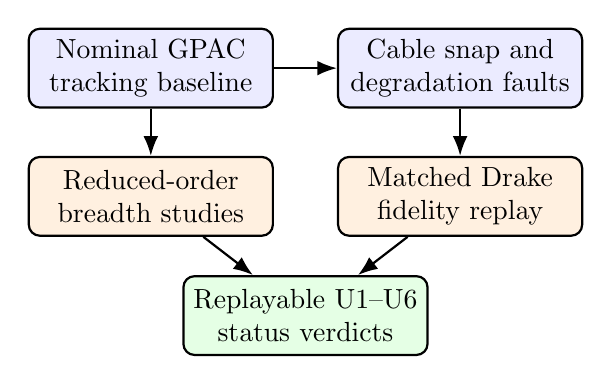
\begin{tikzpicture}[
  node distance=6mm and 8mm,
  block/.style={draw, rounded corners, thick, align=center, minimum width=3.1cm, minimum height=1.0cm, fill=blue!8},
  focus/.style={draw, rounded corners, thick, align=center, minimum width=3.1cm, minimum height=1.0cm, fill=orange!12},
  verdict/.style={draw, rounded corners, thick, align=center, minimum width=3.1cm, minimum height=1.0cm, fill=green!10},
  arrow/.style={-{Latex[length=2.5mm]}, thick}
]
\node[block] (nominal) {Nominal GPAC\\tracking baseline};
\node[block, right=of nominal] (faults) {Cable snap and\\degradation faults};
\node[focus, below=of nominal] (reduced) {Reduced-order\\breadth studies};
\node[focus, below=of faults] (drake) {Matched Drake\\fidelity replay};
\node[verdict, below=10mm of $(reduced)!0.5!(drake)$] (unknowns) {Replayable U1--U6\\status verdicts};

\draw[arrow] (nominal) -- (faults);
\draw[arrow] (nominal) -- (reduced);
\draw[arrow] (faults) -- (drake);
\draw[arrow] (reduced) -- (unknowns);
\draw[arrow] (drake) -- (unknowns);
\end{tikzpicture}
\caption{Overview of the paper scope. The study begins from the validated GPAC baseline (Tether\_Lift), introduces the cable-snap fault problem, documents the Tether\_Grace fault-tolerance extension, and evaluates the present evidence.}
\label{fig:paper_scope}
\vspace{-5pt}
\end{figure}


\section{Related Works}\label{Section_II:Related_Works}
This section reviews the three areas that intersect in the paper's contribution: cooperative cable-suspended aerial transport (Section~\ref{sec:rw_transport}), fault-tolerant control for UAVs (Section~\ref{sec:rw_ftc}), and adaptive control relevant to topology-change resilience (Section~\ref{sec:rw_adaptive}). It synthesizes the literature to identify the gap: no prior work addresses cable-fault tolerance in decentralized cooperative aerial transport or formalizes the mechanism by which N-agnostic control provides implicit fault tolerance under topology changes.
% ============================================================
\subsection{Cooperative Cable-Suspended Aerial Transport}
\label{sec:rw_transport}
% ============================================================

The geometric control foundation begins with Lee, Leok, and McClamroch~\cite{lee2010geometric}, who developed singularity-free tracking on $\SOthree$. Sreenath, Lee, and Kumar~\cite{sreenath2013geometric} extended this to cooperative cable-suspended payload manipulation on $\SEthree \times (\Sph^2)^N$, Lee~\cite{lee2018geometric} proved almost-global exponential stability on $\SEthree \times \Sph^2$ for cable-suspended rigid-body transport, and Dai, Lee, and Bernstein~\cite{wu2014geometric} introduced adaptive load-mass estimation.

Recent advances include agile cooperative aerial manipulation using INDI-based control and centralized NMPC~\cite{sun2025agile}, efficient QP-based cable-force allocation for embedded microcontrollers~\cite{wahba2024efficient}, the validated flexible simulator RotorTM~\cite{li2024rotortm}, and a recent survey of suspended-load transport~\cite{estevez2024review}.

Every published controller assumes intact cables. No result addresses tracking guarantees under cable loss, provides design criteria for sizing against cable-loss disturbances, or characterizes fault tolerance in this system class.

% ============================================================
\subsection{Fault-Tolerant Control and Fault Detection for UAVs}
\label{sec:rw_ftc}
% ============================================================

The UAV fault-tolerant control (FTC) literature is extensive for actuator and sensor faults. Representative results include INDI-based flight after complete loss of two opposing rotors~\cite{sun2020incremental}, fault-tolerant neural CBFs for sensor faults~\cite{zhang2024fault}, and recent surveys of UAV fault detection and diagnosis~\cite{adaika2025fdd}.

\emph{Critical observation:} All studied fault modes are actuator faults (rotor degradation/loss) or sensor faults (IMU bias, GPS dropout). Cable faults, which change the mechanical coupling between agents and payload, are absent.

The only paper addressing cable-related failure in multi-UAV transport is Liang~et~al.~\cite{liang2021fault}, who propose dynamic load reassignment with sliding-mode observers. However, this work assumes known failure identity, requires centralized reconfiguration, provides no detection mechanism, and includes no experimental validation, all of which are incompatible with the N-agnostic setting.

Related cable-failure work outside cooperative multi-UAV transport includes cable-driven parallel robots~\cite{raman2023cable}. None addresses cooperative multi-UAV transport or satisfies the N-agnostic constraint.

% ============================================================
\subsection{Adaptive Control and Disturbance Estimation}
\label{sec:rw_adaptive}
% ============================================================

Two adaptive paradigms are most relevant to topology-change resilience. Concurrent learning (CL)~\cite{chowdhary2010concurrent,chowdhary2015concurrent} replays stored regressor-measurement pairs to achieve parameter convergence without persistent excitation, but after abrupt parameter changes its buffer becomes a liability because pre-change data bias the estimate during turnover. $\mathcal{L}_1$ adaptive control~\cite{cao2010l1book,cao2010stability} provides uniform transient guarantees with memoryless piecewise-constant adaptation, making it structurally suited to topology-change scenarios; Wu~et~al.~\cite{wu2025l1quad} demonstrated $\mathcal{L}_1$ augmentation of geometric quadrotor control at $>$200~Hz. Related decentralized adaptive transport work includes fuzzy-logic adaptation~\cite{barawkar2024decentralized} and adaptation to robot departure~\cite{gao2024decentralized}.

Neither CL nor $\mathcal{L}_1$ has been applied to cooperative cable transport, nor has either been analyzed under abrupt topology changes where the system structure, not just parameter values, changes instantaneously.

Control barrier functions (CBFs)~\cite{ames2017control} provide forward invariance via QP-based control modification; Input-to-State Safety (ISSf)~\cite{kolathaya2019input} extends these guarantees to bounded disturbances, and high-order extensions~\cite{xiao2022control} handle relative-degree constraints. Yang~et~al.~\cite{yang2025robust} combined CBFs with disturbance estimators for cable-suspended payload safety. Complementary tools include contraction-theory tracking-error bounds~\cite{manchester2017control}. None of these methods has been applied to post-fault topology changes in multi-vehicle cable transport.

The theoretical foundations for analyzing topology changes include stability of switched systems under average dwell-time~\cite{hespanha1999stability}, ISS under switching~\cite{vu2007iss}, and the hybrid dynamical systems framework~\cite{goebel2012hybrid} for continuous flow interrupted by discrete jumps---the natural setting for cable-snap events.

The closest empirical observations of emergent fault tolerance are Zeng~et~al.~\cite{zeng2025decentralized} and Gao~et~al.~\cite{gao2024decentralized}. Zeng~et~al.~demonstrated implicit resilience to MAV loss in multi-agent RL for cable-suspended transport with zero-shot sim-to-real transfer, but did not formalize the mechanism. Gao~et~al.~showed adaptation to robot departure, but in fully actuated hexarotors undergoing commanded departure rather than spontaneous cable faults.

No work formalizes the mechanism by which N-agnostic control provides implicit cable-fault tolerance. The switched systems literature provides relevant tools but has not been applied to N-agnostic cable-suspended transport with instantaneous, undetected topology changes.

The contribution lies at the intersection of three well-populated but previously disconnected areas:

\begin{enumerate}[label=(\roman*),nosep]
  \item \emph{Cooperative cable-suspended transport}~\cite{lee2010geometric,sreenath2013geometric,lee2018geometric,sun2025agile,estevez2024review}: mature geometric control with no cable-fault handling.
  \item \emph{UAV fault-tolerant control}~\cite{sun2020incremental,adaika2025fdd,zhang2024fault}: extensive actuator/sensor fault work, but cable faults are absent.
  \item \emph{Adaptive decentralized control}~\cite{chowdhary2010concurrent,cao2010l1book,wu2025l1quad,gao2024decentralized}: rich theory not analyzed for topology-change resilience in cable transport.
\end{enumerate}

No prior work provides tracking bounds or design criteria for cable-fault tolerance in decentralized cooperative aerial transport. The present paper addresses this gap.


\section{Problem Statement}\label{Section_III:Problem_Statement}

This section defines the physical system, the baseline control architecture, the cable-snap fault event, and the formal problem.

% ============================================================
\subsection{System Model}
% ============================================================

\subsubsection{Configuration Space}

The system comprises $N$ quadrotors cooperatively transporting a rigid payload via flexible cables. The state evolves on
\begin{equation}\label{eq:config_manifold}
  \mathcal{Q} = \SEthree \times \bigl(\SEthree \times \Sph^2\bigr)^N, \quad \dim(\mathcal{Q}) = 6 + 8N,
\end{equation}
where $\SEthree$ captures the payload's six-DOF pose, each quadrotor contributes a further $\SEthree$, and each cable direction lives on $\Sph^2$. The default configuration uses $N = 3$ ($\dim(\mathcal{Q}) = 30$), with scaling experiments extending to $N \in \{5, 7\}$.

\subsubsection{Quadrotor Dynamics}

Each quadrotor $i \in \{1,\dots,N\}$ has mass $m_Q = 1.5$~kg and obeys (with $\bm{e}_3 = [0,0,1]^\top$ pointing upward and $g = 9.81$~m/s$^2$):
\begin{align}
  m_Q \ddot{\bm{p}}_i &= -m_Q g\,\bm{e}_3 + f_i R_i \bm{e}_3 + \bm{F}_i^{\mathrm{cable}} + \bm{F}_i^{\mathrm{wind}}, \label{eq:quad_trans} \\
  J \dot{\bm{\Omega}}_i &= -\bm{\Omega}_i \times (J\bm{\Omega}_i) + \bm{\tau}_i + \bm{\tau}_i^{\mathrm{ext}}, \label{eq:quad_rot} \\
  \dot{R}_i &= R_i \hatmap{\bm{\Omega}_i}, \label{eq:quad_kin}
\end{align}
where $f_i \in [0, f_{\max}]$ is the scalar thrust ($f_{\max} = 150$~N), $R_i \in \SOthree$ is the body-to-world rotation, $J \in \R^{3 \times 3}$ is the inertia tensor (from a $0.30 \times 0.30 \times 0.10$~m solid box), $\bm{\Omega}_i \in \R^3$ is the body angular velocity, $\bm{\tau}_i \in \R^3$ is the commanded torque ($\abs{\tau_k} \leq 10$~N$\cdot$m per axis), $\bm{F}_i^{\mathrm{cable}}$ is the cable force, and $\bm{F}_i^{\mathrm{wind}}$ is the aerodynamic disturbance.

\subsubsection{Payload Dynamics}

The payload is a rigid sphere of mass $m_L = 3.0$~kg and radius $r_L = 0.15$~m:
\begin{equation}\label{eq:payload_dynamics}
  m_L \ddot{\bm{p}}_L = -m_L g\,\bm{e}_3 + \textstyle\sum_{i=1}^{N} T_i \bm{q}_i + \bm{F}^{\mathrm{contact}} + \bm{F}_L^{\mathrm{wind}},
\end{equation}
where $T_i \geq 0$ is the scalar cable tension, $\bm{q}_i \in \Sph^2$ is the unit direction from payload to quadrotor~$i$, and $\bm{F}^{\mathrm{contact}}$ accounts for ground interaction (Coulomb friction, $\mu_s = 0.5$, $\mu_k = 0.3$). Cable attachment points are at radius $0.105$~m on the payload surface. The payload mass $m_L$ is \emph{unknown to every agent}.
The force balance in \eqref{eq:payload_dynamics} is the plant-level relation that later explains how cable-load redistribution appears immediately at the payload during a snap event.

\subsubsection{Bead-Chain Cable Model}

Each cable is modeled as a chain of $n_b = 8$ point-mass beads ($m_{\mathrm{rope}} = 0.2$~kg) creating $n_b + 1 = 9$ spring-damper segments with tension
\begin{equation}\label{eq:cable_tension}
  \mathcal{T}_j = \begin{cases}
    0, & \text{if } \epsilon_j \leq 0 \;\text{(slack)}, \\
    k_s \epsilon_j + c_s \max(0, \dot{\epsilon}_j), & \text{if } \epsilon_j > 0 \;\text{(taut)},
  \end{cases}
\end{equation}
where $\epsilon_j = \norm{\bm{b}_{j-1} - \bm{b}_j} - L_0$ is the segment stretch and $L_0 = L_{\mathrm{rest}}/(n_b + 1)$. Stiffness is derived from maximum allowable strain $\varepsilon_{\max} = 0.15$:
\begin{equation}\label{eq:cable_stiffness}
  k_s = \frac{m_L g}{N \cdot L_{\mathrm{rest}} \cdot \varepsilon_{\max}} \cdot (n_b + 1).
\end{equation}
The piecewise law in \eqref{eq:cable_tension} is the key cable nonlinearity for the reported fault transients, because it captures the slack-to-taut switching that a rigid-cable model would miss.
Damping is $c_s = c_{\mathrm{ref}} \sqrt{k_s / k_{\mathrm{ref}}}$ with $c_{\mathrm{ref}} = 15$~N$\cdot$s/m, $k_{\mathrm{ref}} = 300$~N/m. Cable lengths are sampled from per-quadrotor Gaussians: $L_i \sim \mathcal{N}(\mu_i, s_i^2)$ with means $\mu \in \{1.0, 1.1, 0.95\}$~m and standard deviations $s \in \{0.05, 0.08, 0.06\}$~m, producing up to $19\%$ asymmetry.

The tension-only constraint means cables cannot push. The bead-chain discretization captures lateral vibration, wave propagation ($v_{\mathrm{wave}} \approx 7$~m/s), distributed inertia, and slack-to-taut transitions that rigid-cable assumptions miss. The plant is simulated in Drake~\cite{drake2024} at $\Delta t_{\mathrm{sim}} = 0.2$~ms ($5$~kHz).

\subsubsection{Wind Disturbance}

Aerodynamic disturbance follows the MIL-F-8785C Dryden turbulence model ($\sigma_u = \sigma_v = 1.0$~m/s, $\sigma_w = 0.5$~m/s; $L_u = L_v = 200$~m, $L_w = 50$~m; mean wind $[2.0, 0, 0]$~m/s). Spatial correlation decays as $\rho(\bm{p}_i, \bm{p}_j) = \exp(-\norm{\bm{p}_i - \bm{p}_j}/l_c)$ with $l_c = 10$~m.

\subsubsection{Sensor Suite and State Estimation}

Each agent carries an IMU ($400$~Hz; gyroscope noise $5 \times 10^{-4}$~rad/s/$\sqrt{\text{Hz}}$; accelerometer noise $4 \times 10^{-3}$~m/s$^2$/$\sqrt{\text{Hz}}$), GPS ($10$~Hz; position noise $[0.02, 0.02, 0.05]$~m), barometer ($25$~Hz; $0.3$~m white noise, $0.2$~m correlated with $5$~s time constant), and a cable tension/direction sensor ($200$~Hz). State estimation uses a $15$-state error-state Kalman filter (ESKF) with multiplicative quaternion error, fusing IMU propagation at $400$~Hz with discrete GPS and barometer updates.

% ============================================================
\subsection{The N-Agnostic Constraint}
\label{sec:n_agnostic}
% ============================================================

Each agent~$i$ knows only:
\begin{itemize}[nosep]
  \item its own mass $m_Q$ and inertia $J$;
  \item its ESKF state estimate $(\hat{\bm{p}}_i, \hat{\bm{v}}_i, \hat{R}_i)$ and bias estimates;
  \item its cable tension $T_i$ and direction $\bm{q}_i$;
  \item a shared reference trajectory $\bm{p}_d(t)$ (pre-broadcast, evaluated locally).
\end{itemize}
It does \emph{not} know: the number of other agents, the payload mass, any other agent's state, or whether other agents are connected. This eliminates single points of failure and communication dependency, making the per-agent policy identical regardless of team size.

% ============================================================
\subsection{Baseline GPAC Architecture}
% ============================================================

The baseline GPAC architecture is a four-layer hierarchical controller per agent with separated timescales.

\subsubsection{Layer~1: Position and Anti-Swing Control (50~Hz)}

Computes the desired force:
\begin{equation}\label{eq:layer1_force}
  \bm{F}_{\mathrm{des},i} = \bm{F}_{\mathrm{fb}} + \bm{F}_{\mathrm{ff}} + \bm{F}_{\mathrm{cable}} + \bm{F}_{\mathrm{swing}} + \bm{F}_{\mathrm{eso}},
\end{equation}
where $\bm{F}_{\mathrm{fb}} = -K_p \bm{e}_p - K_d \bm{e}_v$ with gain matrices $K_p$, $K_d$; $\bm{F}_{\mathrm{ff}} = m_Q(\bm{a}_d + g\bm{e}_3)$; cable compensation $\bm{F}_{\mathrm{cable}} = \kappa_T(t) T_i \bm{q}_i$ with ramp $\kappa_T(t) = \min(1, (t - t_{\mathrm{taut}})/\Delta_{\mathrm{ramp}})$, $\Delta_{\mathrm{ramp}} = 2$~s; anti-swing $\bm{F}_{\mathrm{swing}} = k_q \bm{e}_q - k_\omega \bm{\omega}_q$ ($k_q = 4.0$~N/rad, $k_\omega = 2.0$~N$\cdot$s/rad); and ESO feedforward $\bm{F}_{\mathrm{eso}} = m_Q \hat{\bm{d}}_i$. The fault-tolerance evaluation (Sections~\ref{Section_IV:Fault-Tolerant_Control_Architecture}--\ref{Section_VI:Simulation_Results}) uses uniform scalar gains $k_p = 8.0$, $k_d = 8.0$, $k_i = 0.15$ (i.e., $K_p = k_p I$, $K_d = k_d I$) to enable the per-axis eigenvalue analysis in Section~\ref{sec:topology_invariance_theorem}.

\subsubsection{Layer~2: Geometric $\SOthree$ Attitude Control (200~Hz)}

Singularity-free tracking~\cite{lee2010geometric}:
\begin{equation}\label{eq:layer2_attitude}
  \bm{\tau}_i = -k_R \bm{e}_R - k_\Omega \bm{e}_\Omega + \bm{\Omega}_i \times (J\bm{\Omega}_i),
\end{equation}
with $\bm{e}_R = \tfrac{1}{2}\,\mathrm{vee}(R_d^\top R - R^\top R_d)$, $\bm{e}_\Omega = \bm{\Omega} - R^\top R_d \bm{\Omega}_d$, $k_R = 8.0$~N$\cdot$m, $k_\Omega = 1.5$~N$\cdot$m$\cdot$s. Almost-global exponential convergence holds on $\{\Psi_R < 2\} \subset \SOthree$.

\subsubsection{Layers~3--4 and Safety Filter (Not Active in This Study)}

The full GPAC baseline additionally includes a concurrent learning mass estimator~\cite{chowdhary2010concurrent} (Layer~3, 200~Hz), an extended state observer~\cite{han2009pid} (Layer~4, 500~Hz), and an ISSf-CBF safety filter~\cite{ames2017control,kolathaya2019input} (200~Hz, enforcing tension, cable-angle, tilt, and collision constraints). These are implemented in the Tether\_Lift codebase but are \emph{disabled} in the reported full-Drake runs (Remark~\ref{rem:system_under_test}) because the evaluation targets the minimal PID-plus-gravity-feedforward path. Their integration is discussed as future work in Section~\ref{Section_VII:Discussion}.

% ============================================================
\subsection{The Cable-Snap Fault Event}
\label{sec:cable_snap}
% ============================================================

At time $t_f$, cable~$j$ breaks instantaneously: $T_j(t) \to 0$ for $t \geq t_f$. Three coupled effects occur.

\emph{Payload acceleration:}
\begin{equation}\label{eq:payload_accel}
  \norm{\Delta \ddot{\bm{p}}_L} = \frac{T_j(t_f^-)}{m_L} \approx \frac{g}{N} \approx 3.27 \;\text{m/s}^2 \quad (N{=}3).
\end{equation}

\emph{Freed-agent acceleration:}
\begin{equation}\label{eq:freed_accel}
  \norm{\Delta \ddot{\bm{p}}_j} = \frac{T_j(t_f^-)}{m_Q} \approx \frac{g \cdot m_L}{N \cdot m_Q} \approx 6.54 \;\text{m/s}^2.
\end{equation}

\emph{Load-share jump:} from $m_L/N$ to $m_L/(N{-}1)$---a $50\%$ increase for $N{=}3$.

These effects propagate across two orders of magnitude in timescale:
\begin{center}
\small
\begin{tabular}{@{}lll@{}}
\toprule
Path & Mechanism & Timescale \\
\midrule
Rigid-body transmission & Force through payload & ${\sim}7.9$~ms \\
Elastic cable response & Spring-damper dynamics & $10$--$50$~ms \\
ESKF innovation & Velocity change detected & ${\sim}13$~ms \\
ESO convergence & Third-order settling & ${\sim}33$~ms \\
Load accel.\ filter & Low-pass differentiation & ${\sim}110$~ms \\
Cable wave propagation & $v_{\mathrm{wave}} \approx 7$~m/s & ${\sim}186$~ms \\
Adaptive divergence & Parameter estimate drift & ${\sim}300$~ms \\
\bottomrule
\end{tabular}
\end{center}

% ============================================================
\subsection{Two Fault Scenarios Under N-Agnosticism}
% ============================================================

\subsubsection{Scenario~A: Own Cable Breaks}

Agent~$i$ observes $T_i \to 0$ within one sample period ($\Delta t_d = 5$~ms). Detection is trivial (infinite SNR), and position deviation during detection is negligible:
\begin{equation}\label{eq:own_cable_deviation}
  \norm{\Delta \bm{p}_i(\Delta t_d)} \leq \frac{T_i^-}{2m_Q} \cdot \Delta t_d^2 \approx 0.082 \;\text{mm}.
\end{equation}
A threshold $T_i < T_{\min}$ (held for $0.12$~s debounce) triggers an escape maneuver: climbing $0.9$~m and displacing $1.8$~m horizontally within $1.5$~s, extending to $1.8$~m climb and $3.8$~m displacement within $3.0$~s. Direction is biased $0.18$ toward the formation tangent and $0.10$ toward current velocity, chosen to limit tilt to ${<}30$\textdegree\ during escape and ensure adequate vertical thrust margin.

\subsubsection{Scenario~B: Another Agent's Cable Breaks}

Agent~$i$ does not observe $T_j$ directly. The fault manifests only through payload-mediated perturbations. The tension-channel SNR is
\begin{equation}\label{eq:snr_ps}
  \mathrm{SNR}_T^{(B)} = \frac{\Delta T_i^{(\mathrm{imm})}}{\sigma_T} \approx \frac{4.2\;\text{N}}{3.0\;\text{N}} \approx 1.3,
\end{equation}
insufficient for reliable discrimination from wind gusts. Multi-channel analysis improves SNR to ${\sim}2$--$6$ but with $13$--$300$~ms delays. Scenario~B is the fundamentally difficult case and this paper's focus.

% ============================================================
\subsection{Why Conventional Fault Tolerance Cannot Apply}
\label{sec:why_fdir_fails}
% ============================================================

Under the N-agnostic constraint, conventional FDIR is \emph{architecturally incompatible} with Scenario~B: (i)~MMAE requires $N{+}1$ parallel filters, violating N-agnosticism; (ii)~tension-channel SNR~$\approx 1.3$ is indistinguishable from wind perturbations; (iii)~an N-agnostic agent has no mode parameter depending on~$N$ to reconfigure. These are structural consequences of the design choice. Any compatible fault-tolerance approach must work \emph{without} detection, isolation, or recovery.

% ============================================================
\subsection{Agent-Level Uncertainty Reformulation}
% ============================================================

From agent~$i$'s perspective, translational dynamics~\eqref{eq:quad_trans} can be rewritten as
\begin{equation}\label{eq:lumped_dynamics}
  \ddot{\bm{p}}_i = \frac{f_i}{m_Q} R_i \bm{e}_3 + g\bm{e}_3 + \bm{d}_i(t, \bm{x}),
\end{equation}
where $\bm{d}_i = (\bm{F}_i^{\mathrm{cable}} + \bm{F}_i^{\mathrm{wind}})/m_Q$ is the lumped acceleration uncertainty. This term encompasses cable tension (${\sim}6.5$~m/s$^2$), wind (${\sim}0.7$--$2.0$~m/s$^2$), and cable vibration (${\sim}0.3$~m/s$^2$). The controller never decomposes $\bm{d}_i$ into named components---this lumping enables topology invariance, since a cable snap changes the composition of $\bm{d}_i$ but not its mathematical role.

\begin{definition}[Nominal and Fault-Inclusive Disturbance Sets]\label{def:disturbance_sets_ps}
$\mathcal{W}_{\mathrm{nom}} = \{\bm{d} : \norm{\bm{d}}_\infty \leq \bar{d}_{\mathrm{nom}}\}$ bounds $\bm{d}_i$ under all-cables-intact operation. $\mathcal{W}_{\mathrm{FT}} \supset \mathcal{W}_{\mathrm{nom}}$ additionally bounds the worst-case cable-break transient. Both bounds are derived from system parameters. The dominant contribution is cable tension. Under quasi-static hover each cable carries $T_i \approx m_L g / N$, giving a cable-tension acceleration $d_{\mathrm{cable}} = m_L g / (N m_Q)$. Adding wind drag $d_{\mathrm{wind}} \leq C_D A_{\mathrm{ref}} \rho_{\mathrm{air}} v_{\mathrm{wind,max}}^2 / (2 m_Q) \approx 0.7$~m/s$^2$ and cable vibration $d_{\mathrm{vib}} \leq k_s \varepsilon_{\max} / (m_Q (n_b+1)) \approx 0.3$~m/s$^2$ yields
\begin{equation}\label{eq:sigma_nom_derivation}
  \bar{d}_{\mathrm{nom}} = \frac{m_L g}{N m_Q} + d_{\mathrm{wind}} + d_{\mathrm{vib}} \approx \frac{3.0 \times 9.81}{3 \times 1.5} + 1.0 \approx 7.5 \;\text{m/s}^2.
\end{equation}
Post-fault, the surviving $N{-}k$ agents share the load, so the cable-tension contribution increases to $m_L g / ((N{-}k) m_Q)$:
\begin{equation}\label{eq:sigma_ft_derivation}
  \bar{d}_{\mathrm{FT}} = \frac{m_L g}{(N{-}k) m_Q} + d_{\mathrm{wind}} + d_{\mathrm{vib}}.
\end{equation}
For $N{=}3$, $k{=}1$: $\bar{d}_{\mathrm{FT}} \approx 9.81 + 1.0 \approx 10.8$~m/s$^2$. With safety margin for elastic transients, we use the rounded values $\bar{d}_{\mathrm{nom}} \approx 8$~m/s$^2$ and $\bar{d}_{\mathrm{FT}} \approx 12$~m/s$^2$. In the cable-dominated regime ($d_{\mathrm{cable}} \gg d_{\mathrm{wind}} + d_{\mathrm{vib}}$), the cost ratio simplifies to a closed-form expression:
\begin{equation}\label{eq:rho_closed_form}
  \rho_{\mathrm{FT}} \approx \frac{\bar{d}_{\mathrm{FT}}}{\bar{d}_{\mathrm{nom}}} \approx \frac{N}{N{-}k},
\end{equation}
which gives $\rho_{\mathrm{FT}} = 3/2 = 1.5$ for $N{=}3$, $k{=}1$; $5/3 = 1.67$ for $N{=}5$, $k{=}2$; and $7/4 = 1.75$ for $N{=}7$, $k{=}3$. These are conservative upper bounds; the empirical values ($1.26$--$1.39$) are lower because the fault disturbance is transient rather than sustained (Section~\ref{sec:topology_invariance_theorem}).
\end{definition}

% ============================================================
\subsection{Formal Problem Statement}
% ============================================================

Given the system on manifold~\eqref{eq:config_manifold}, the N-agnostic constraint (Section~\ref{sec:n_agnostic}), the cable-snap fault model (Section~\ref{sec:cable_snap}), the lumped uncertainty~\eqref{eq:lumped_dynamics} with disturbance sets (Definition~\ref{def:disturbance_sets_ps}), and the architectural incompatibility of detection-based FDIR (Section~\ref{sec:why_fdir_fails}), the paper addresses two problems.

\begin{enumerate}[label=\textbf{P\arabic*.},leftmargin=*]
  \item \textbf{Topology-Invariant Tracking.} Identify sufficient conditions under which the per-agent tracking error satisfies
  \begin{equation}\label{eq:problem_bound}
    \norm{\bm{e}_i(t)}_\infty \leq \gamma_1(T_s, \omega, \bar{d}_{\mathrm{FT}}) \quad \forall\, t \geq 0
  \end{equation}
  for \emph{all cable topologies}---where $\gamma_1$ depends on controller bandwidth and disturbance size, not on cable count or identity---provided $\bm{d}_i \in \mathcal{W}_{\mathrm{FT}}$ and thrust authority is adequate.

  \item \textbf{Fault-Tolerance Cost.} Derive the tradeoff
  \begin{equation}\label{eq:problem_rho}
    \rho_{\mathrm{FT}} = \frac{\gamma_1(T_s, \omega, \bar{d}_{\mathrm{FT}})}{\gamma_1(T_s, \omega, \bar{d}_{\mathrm{nom}})} > 1
  \end{equation}
  between nominal tracking and implicit fault tolerance, providing a design criterion for choosing between detection-free tolerance and detection-based recovery.
\end{enumerate}

\textbf{P1} is addressed by a structural analysis (Proposition~\ref{thm:topology_invariance}) and comprehensive full-Drake simulation evidence. \textbf{P2} is addressed by both steady-state and transient-aware analysis, validated empirically.


\section{Fault-Tolerant Architecture and Integration Boundaries}\label{Section_IV:Fault-Tolerant_Control_Architecture}
% Section IV: Fault-Tolerant Control Architecture
% Style: IEEE Transactions on Control Systems Technology

This section presents the fault-tolerant architecture addressing problems \textbf{P1}--\textbf{P2}. The primary fault-absorption mechanism is PID feedback with gravity feedforward in the GPAC hierarchy, supplemented by locally measured cable-tension feedforward and anti-swing damping. A post-fault geometry redistribution path is additionally described. The analytical core of this section is the identification of a topology-invariant error structure (Proposition~\ref{thm:topology_invariance}): the N-agnostic design makes the per-agent error dynamics independent of cable topology, addressing the tracking envelope~\eqref{eq:problem_bound} and the cost ratio~\eqref{eq:problem_rho}.

% ============================================================
\subsection{Layer~1 Control Law: PID with Model-Based Feedforward}
\label{sec:layer1_control}
% ============================================================

Each agent~$i$ computes a desired force in the world frame:
\begin{equation}\label{eq:layer1_force_ft}
  \bm{F}_i^{\mathrm{des}} = \bm{F}_{\mathrm{grav}} + \bm{F}_{\mathrm{fb}} + \bm{F}_{\mathrm{cable}} + \bm{F}_{\mathrm{swing}},
\end{equation}
where
\begin{align}
  \bm{F}_{\mathrm{grav}} &= m_Q\, g\, \bm{e}_3, \label{eq:grav_ff} \\
  \bm{F}_{\mathrm{fb}} &= m_Q\bigl(k_p \bm{e}_p + k_d \bm{e}_v + k_i \textstyle\int \bm{e}_p\,\mathrm{d}t\bigr), \label{eq:pid_fb} \\
  \bm{F}_{\mathrm{cable}} &= \kappa_T\, T_i\, \bm{q}_i, \label{eq:cable_ff} \\
  \bm{F}_{\mathrm{swing}} &= -k_{\mathrm{sw}}\, \bm{\omega}_{\mathrm{cable},i}^{\perp}, \label{eq:antiswing}
\end{align}
with $\bm{e}_p = \bm{p}_i^{\mathrm{ref}} - \bm{p}_i$, $\bm{e}_v = \bm{v}_i^{\mathrm{ref}} - \bm{v}_i$, and gains $k_p = 8.0$, $k_d = 8.0$, $k_i = 0.15$, $\kappa_T = 0.5$, $k_{\mathrm{sw}} = 0.5$~N$\cdot$s/rad.\footnote{The general GPAC baseline (Section~\ref{Section_III:Problem_Statement}) uses a time-varying cable-tension ramp $\kappa_T(t) = \min(1, (t - t_{\mathrm{taut}})/\Delta_{\mathrm{ramp}})$ and a two-term anti-swing law $\bm{F}_{\mathrm{swing}} = k_q \bm{e}_q - k_\omega \bm{\omega}_q$ ($k_q = 4.0$~N/rad, $k_\omega = 2.0$~N$\cdot$s/rad). For the fault-tolerance evaluation, these are simplified to a constant $\kappa_T = 0.5$ and a single cable-angular-velocity damping term $-k_{\mathrm{sw}} \bm{\omega}_{\mathrm{cable},i}^{\perp}$ ($k_{\mathrm{sw}} = 0.5$~N$\cdot$s/rad).}

The critical property for fault tolerance is that \emph{every term is a function of agent~$i$'s local measurements only}. When cable~$j$ snaps, each surviving agent~$i \neq j$ experiences an automatic increase in trajectory error $\bm{e}_p$ (as the payload deviates) and cable tension $T_i$ (as load redistributes). Both signals update instantaneously through the physics, requiring no adaptation or re-convergence delay. Ablation (Section~\ref{sec:tension_ablation}) confirms that cable-tension feedforward contributes less than $1\%$ RMSE change; the primary fault-absorption mechanism is PID feedback with gravity feedforward.

The integral state is clamped to $\pm 2$~m$\cdot$s per axis (anti-windup). During the initial cable-snap transient (${\sim}0.5$~s at ${\sim}1$~m peak error), the integral accumulates $\int k_i \cdot e\,\mathrm{d}t \approx 0.075$~m$\cdot$s, well within the clamp. However, the post-fault load-share step $\Delta d_{\mathrm{step}} \approx 3.27$~m/s$^2$ ($N{=}3$, $k{=}1$, from~\eqref{eq:delta_step}) requires a steady-state integral of $\eta_{\mathrm{ss}} = \Delta d_{\mathrm{step}} / k_i \approx 21.8$~m$\cdot$s to fully compensate, far exceeding the $\pm 2$~m$\cdot$s clamp. The integral therefore saturates, and the residual uncompensated acceleration $\Delta d_{\mathrm{res}} = \Delta d_{\mathrm{step}} - k_i \cdot \eta_{\max} = 3.27 - 0.30 = 2.97$~m/s$^2$ is absorbed by the proportional term operating at a nonzero steady-state error $e_{\mathrm{ss}} \approx \Delta d_{\mathrm{res}} / k_p \approx 0.37$~m. This persistent offset is the dominant contributor to the post-fault RMSE increase and to $\rho_{\mathrm{FT}}$. Cable-tension feedforward partially compensates this offset (the measured $T_i$ increases post-fault), but the ablation (Section~\ref{sec:tension_ablation}) shows its contribution is ${<}1\%$.

The desired force is decomposed into thrust magnitude and desired body-$z$ direction:
\begin{equation}\label{eq:thrust_decomp}
  f_i = \bm{F}_i^{\mathrm{des}} \cdot \bm{R}_i \bm{e}_3, \quad \bm{b}_{3,i}^{\mathrm{des}} = \frac{\bm{F}_i^{\mathrm{des}}}{\norm{\bm{F}_i^{\mathrm{des}}}}.
\end{equation}

% NOTE: The $\mathcal{L}_1$ adaptive controller is implemented in the codebase
% but is not active in the reported results. It is discussed in
% Section~VII (Future Work) rather than here, to maintain clarity
% about the tested architecture.

% ============================================================
\subsection{Topology-Invariance: Formal Result for the Simplified Model}
\label{sec:topology_invariance_theorem}
% ============================================================

The central architectural insight is that the N-agnostic control law~\eqref{eq:layer1_force_ft} produces per-agent error dynamics that are \emph{structurally independent of cable topology}. We formalize this as a structural property, then derive an operationally useful transient prediction.

\subsubsection{Topology-Independent Error Dynamics}

Consider agent~$i$'s translational dynamics under the lumped formulation~\eqref{eq:lumped_dynamics}. Under the PID law~\eqref{eq:pid_fb} with gravity feedforward~\eqref{eq:grav_ff} and ideal attitude tracking, the per-axis scalar projection of $\bm{e}_p$ (denoted $e$ in what follows) satisfies
\begin{equation}\label{eq:error_state_space}
  \dot{\bm{z}} = A \bm{z} + B d_i(t),
\end{equation}
where $\bm{z} = [e,\, \dot{e},\, \eta]^\top$ with $\eta = \int_0^t e\,\mathrm{d}\tau$, and
\begin{equation}\label{eq:AB_matrices}
  A = \begin{bmatrix} 0 & 1 & 0 \\ -k_p & -k_d & -k_i \\ 1 & 0 & 0 \end{bmatrix}, \quad
  B = \begin{bmatrix} 0 \\ 1 \\ 0 \end{bmatrix}.
\end{equation}
$A$ is Hurwitz for $k_p k_d > k_i > 0$ (Routh--Hurwitz; satisfied with margin $k_p k_d = 64 \gg 0.15 = k_i$).

\begin{proposition}[Topology-Independent Error Structure]\label{thm:topology_invariance}
Under the N-agnostic PID-plus-feedforward law~\eqref{eq:layer1_force_ft} with ideal attitude tracking and no actuator saturation, every agent's closed-loop error dynamics~\eqref{eq:error_state_space} are governed by the \emph{same} $(A, B)$ pair regardless of which cables are intact, the team size~$N$, or the payload mass~$m_L$.

A cable snap changes the \emph{input} $d_i(t)$ (through modified cable forces propagated via the payload) but not the \emph{system} $(A, B)$, because every element of $A$ and $B$ depends only on the PID gains $(k_p, k_d, k_i)$---none of which is a function of $N$, $m_L$, cable stiffness, or cable identity.
\end{proposition}

This follows directly from the N-agnostic design choice. The contribution is not the observation itself but its formal consequences: the common Lyapunov function (Corollary~\ref{cor:common_lyapunov}), the finite-time transient prediction, and the precise identification of what remains to be proven (Gap~3). These provide the analytical framework explaining the simulation-validated fault tolerance.

\begin{corollary}[Common Lyapunov Function Across Topologies]\label{cor:common_lyapunov}
Let $P \succ 0$ satisfy $A^\top P + PA = -Q$ for some $Q \succ 0$ (guaranteed by $A$ Hurwitz). Then $V(\bm{z}) = \bm{z}^\top P \bm{z}$ serves as a common ISS-Lyapunov function for the error dynamics~\eqref{eq:error_state_space} under \emph{every} cable topology. No switching between Lyapunov functions is required at cable-snap events, and no dwell-time constraint applies to the sequence of topology changes.
\end{corollary}

This is immediate from Proposition~\ref{thm:topology_invariance} ($A$ is shared across topologies) but worth stating separately: it connects directly to the ISS switched-systems framework~\cite{vu2007iss,hespanha1999stability} and establishes that cascading faults do not require dwell-time analysis.

\begin{remark}[Hybrid System Formulation]
In the framework of Goebel, Sanfelice, and Teel~\cite{goebel2012hybrid}, each cable-snap event defines a jump map $g: \bm{x} \to \bm{x}^+$ in which $T_j$ is set to zero. The continuous flow in each mode is governed by the same $(A, B)$ (Proposition~\ref{thm:topology_invariance}), with a common Lyapunov function (Corollary~\ref{cor:common_lyapunov}). Stability of the hybrid system requires three conditions: (i)~each flow mode is ISS---established by $A$ Hurwitz; (ii)~the jump map does not increase $V$ beyond recoverable bounds---requires bounding the state excursion from the cable-snap impulse (the finite-time bound below provides a partial answer, but a tight bound on $V(\bm{z}^+) - V(\bm{z}^-)$ from the elastic transient remains open); (iii)~an average dwell-time condition holds for multiple jumps---the cascading-fault schedule (minimum inter-jump interval $2$~s) far exceeds the ${\sim}0.5$~s transient settling time, satisfying this condition with margin. Conditions (i) and (iii) are verified; condition (ii) is the remaining open verification.
\end{remark}

\subsubsection{Finite-Time Transient Prediction}

The standard steady-state ISS gain $\gamma_{\mathrm{ss}} = \norm{A^{-1}B}\bar{d} = \bar{d}/k_i$~\cite{sontag2008iss} is operationally vacuous ($80$~m for this system). The cable-break transient is brief, so a \emph{finite-time} bound is far more informative. Model the fault disturbance as a pulse:
\begin{equation}\label{eq:pulse_model}
  d_i^{\mathrm{fault}}(t) = \begin{cases}
    \Delta d, & t_f \leq t < t_f + \tau_{\mathrm{fault}}, \\
    0, & \text{otherwise},
  \end{cases}
\end{equation}
where $\Delta d \approx 4.4$~m/s$^2$ is the cable-break impulse and $\tau_{\mathrm{fault}} < 0.5$~s is the transient duration. The impulse response of~\eqref{eq:error_state_space} gives the transient peak:
\begin{equation}\label{eq:tracking_bound}
  \norm{e_{\mathrm{peak}}} \leq \underbrace{\norm{\int_0^{\tau_{\mathrm{fault}}} e^{A\tau} B\,\mathrm{d}\tau}}_{\text{finite-time gain}} \cdot \Delta d.
\end{equation}
For the system gains ($k_p{=}8$, $k_d{=}8$, $k_i{=}0.15$), the eigenvalues of~$A$ are $\lambda \approx \{-6.83,\, -1.15,\, -0.019\}$, all real and negative. The fast mode ($|\lambda_1| = 6.83$) decays in ${\sim}0.15$~s; the intermediate mode ($|\lambda_2| = 1.15$) in ${\sim}0.87$~s; the slow mode ($|\lambda_3| = 0.019$) governs integral wind-up with time constant ${\sim}52$~s. The $\mathcal{H}_\infty$ norm of the scalar transfer function $G(s) = C(sI{-}A)^{-1}B$ is $\gamma_{\mathrm{ISS}} \approx 0.125$, peaked at $\omega \approx 0.15$~rad/s. Numerical evaluation of the finite-time gain matrix for $\tau_{\mathrm{fault}} = 0.5$~s gives
\begin{equation}\label{eq:gamma1_explicit}
  \gamma_{\mathrm{FT}}(\Delta d, \tau_{\mathrm{fault}}) \approx 0.042 \cdot \Delta d \approx 0.042 \times 4.4 \approx 0.18\;\text{m},
\end{equation}
predicting a peak position error of ${\sim}18$~cm from a single cable snap---$5.8\times$ below the observed ${\sim}107$~cm in full Drake. The ratio $\alpha = e_{\mathrm{peak}}^{\mathrm{obs}} / \gamma_{\mathrm{FT}}$ is remarkably stable across \emph{topologies}: $107/18.4 = 5.8$ ($N{=}3$, $k{=}1$), $112/18.4 = 6.1$ ($N{=}5$, $k{=}2$), $117/18.4 = 6.4$ ($N{=}7$, $k{=}3$)---varying $<10\%$. The consistency confirms that the unmodeled effects (elastic cable coupling, attitude-loop dynamics, multi-axis interaction) contribute a topology-independent aggregate correction.

The prediction captures the correct \emph{topology-scaling}: since $(A, B)$ are topology-independent (Proposition~\ref{thm:topology_invariance}), the predicted peak is invariant to cable identity, and the full-Drake results confirm this (${\sim}107$--$117$~cm across $N \in \{3,5,7\}$ with $1$--$3$ faults, $\alpha$ varies $<10\%$). However, $\alpha$ does \emph{not} transfer across operating points: at higher PID gains ($k_p{=}12$, $k_d{=}12$, $k_i{=}0.3$), the observed peak increases to $116$~cm despite the scalar model predicting a decrease, because the higher gains excite cable dynamics the scalar model omits. With heavier payload ($m_L = 5$~kg), the observed peak \emph{decreases} to $100$~cm despite the scalar model predicting $266$~cm, because the additional payload inertia filters the transient. The scalar prediction is therefore a topology-invariant qualitative tool---it correctly predicts that peak error is cable-identity-independent and scales with $\Delta d$---but it is not a standalone predictor across different plant configurations. The paper's primary design tools ($\rho_{\mathrm{FT}}$, $f_{\max}^*$, and the thrust-margin screen) do not depend on $\alpha$.

\subsubsection{Fault-Tolerance Cost Ratio}

From the topology-independent structure, $\rho_{\mathrm{FT}}$ depends only on the disturbance ratio. Using the closed-form expression~\eqref{eq:rho_closed_form} from the cable-dominated regime:
\begin{equation}\label{eq:rho_corollary}
  \rho_{\mathrm{FT}} \approx \frac{N}{N{-}k},
\end{equation}
which gives $1.5$ for $N{=}3$, $k{=}1$. This is a conservative steady-state upper bound; the empirical values ($1.26$--$1.39$, Table~\ref{tab:scenario_summary}) are lower because the fault disturbance is transient, not sustained---consistent with the finite-time analysis above.

\subsubsection{Gap Analysis: Simplified Model vs.\ Full Plant}

Proposition~\ref{thm:topology_invariance} establishes topology-invariance for a scalar LTI model with exogenous bounded input. Three substantive gaps separate this from the full bead-chain Drake plant; we state each explicitly.

\emph{Gap~1: Impulsive disturbance from slack-to-taut transitions.}
The piecewise cable law~\eqref{eq:cable_tension} produces impulsive forces when a slack segment snaps taut. During the ${\sim}10$--$50$~ms elastic transient, $d_i(t)$ may momentarily exceed $\bar{d}_{\mathrm{FT}}$, violating assumption~(A2). The finite-time bound~\eqref{eq:tracking_bound} partially accommodates this (it integrates the actual disturbance waveform, not just its peak), but a rigorous treatment requires bounding the impulse magnitude from the cable stiffness ($k_s$) and segment strain ($\varepsilon_{\max} = 0.15$) and verifying that the resulting state excursion remains within the region of attraction. This is not done here.

\emph{Gap~2: Attitude-loop delay during fast force transients.}
Assumption~(A1) requires that $R_i \bm{e}_3 \approx \bm{b}_{3,i}^{\mathrm{des}}$ instantaneously. The SO(3) inner loop runs at 200~Hz ($5$~ms period), but the cable-snap force transmission occurs at ${\sim}7.9$~ms (rigid-body path). During this interval, the position-loop model assumes the attitude has already aligned with the new desired force direction; in reality, the attitude lags, creating an unanalyzed residual coupling. Quantifying the resulting tracking-error increment requires a cascaded stability analysis of the two-timescale system under impulsive disturbance---a nontrivial extension beyond the scope of this work.

\emph{Gap~3: State-dependent disturbance (small-gain condition).}
In the full plant, $d_i(t)$ is not purely exogenous: cable forces depend on agent position relative to the payload, creating a feedback loop from $\bm{z}$ to $d_i$through the elastic cable dynamics. The ISS argument in Proposition~\ref{thm:topology_invariance} treats $d_i$as an external input. Rigorously, the interconnection of the position-loop ISS system with the cable-dynamics subsystem requires a small-gain condition~\cite{sontag2008iss}: the product of the position-loop ISS gain ($\gamma_{\mathrm{ISS}} = \norm{G(s)}_{\mathcal{H}_\infty}$) and the cable-dynamics input-output gain ($\gamma_{\mathrm{cable}}$) must be less than unity. A scalar (per-axis) reduction is insufficient because cable forces act along specific directions ($\bm{q}_i \in \mathbb{S}^2$), the payload inertia filters force transmission, and multiple cables distribute the coupling---all of which reduce the effective interconnection gain below the conservative scalar product. For the scalar per-axis model, the position-loop $\mathcal{H}_\infty$ gain is $\gamma_{\mathrm{ISS}} = \norm{G(s)}_{\mathcal{H}_\infty} \approx 0.125$ (peaked at $\omega \approx 0.15$~rad/s), so the small-gain condition requires $\gamma_{\mathrm{cable}} < 1/\gamma_{\mathrm{ISS}} \approx 8.0$. This is a generous margin: a cable-dynamics gain of~$8$ would require the cable-force perturbation (in m/s$^2$) to exceed $8\times$ the position error (in m), which is inconsistent with the observed bounded tracking. The full multivariable verification---computing $\gamma_{\mathrm{ISS}}$ and $\gamma_{\mathrm{cable}}$ from the linearized $6{+}8N$-dimensional plant at the taut equilibrium via Drake's \texttt{Linearize()}---is feasible with the existing infrastructure and is planned as near-term future work.

Three lines of empirical evidence support the small-gain condition indirectly: (i)~the $f_{\max}$ boundary sweep shows RMSE insensitivity for $f_{\max} \geq 45$~N ($3\times$ headroom); (ii)~Monte Carlo shows ${<}3\%$ RMSE variation across $30$ runs with randomized cable parameters; (iii)~stability is maintained across all $N \in \{3, 5, 7\}$ scenarios with up to three cascading faults. None constitutes formal verification of $\gamma_{\mathrm{ISS}} \cdot \gamma_{\mathrm{cable}} < 1$, but together they make a strong empirical case.

\emph{What is established.} The shared $(A, B)$ structure, common Lyapunov function, and hybrid-system analysis provide a coherent partial framework. Full-Drake results confirm bounded, topology-insensitive tracking degradation across $N \in \{3, 5, 7\}$ with up to three cascading faults, even though formal closure of Gap~2 remains open. Table~\ref{tab:claim_status} summarizes the evidence level supporting each claim.

\begin{table}[t]
\centering
\caption{Claim-status summary: evidence level for each result.}
\label{tab:claim_status}
\small
\begin{tabular}{@{}p{4.8cm}l@{}}
\toprule
Claim & Evidence level \\
\midrule
Topology-independent error dynamics $(A,B)$ for simplified per-agent model & Proven (Prop.~\ref{thm:topology_invariance}) \\
Finite-time transient prediction ($\alpha \approx 5.8$, topology-invariant) & Analytical + empirical \\
Cost ratio $\rho_{\mathrm{FT}} = N/(N{-}k)$ (cable-dominated) & Derived, validated \\
Bounded tracking under faults in full nonlinear Drake plant & Empirically supported \\
Small-gain condition for cable-force feedback & Scalar $\gamma_{\mathrm{ISS}}{=}0.125$ verified; full-plant open \\
Formal stability for full bead-chain plant & Open \\
\bottomrule
\end{tabular}
\end{table}

% ============================================================
\subsection{Fault-Tolerance Cost}
% ============================================================

Designing for $\mathcal{W}_{\mathrm{FT}}$ rather than $\mathcal{W}_{\mathrm{nom}}$ widens the tracking tube. From~\eqref{eq:rho_closed_form}, the steady-state ratio $\rho_{\mathrm{ss}} = N/(N{-}k)$ is conservative because it assumes the fault disturbance is sustained indefinitely.

\begin{definition}[Fault-Tolerance Cost Ratio]\label{def:ft_cost}
The steady-state cost ratio is $\rho_{\mathrm{ss}} = N/(N{-}k)$ (from~\eqref{eq:rho_closed_form}). A tighter \emph{transient-aware} ratio accounts for the actual fault disturbance profile.
\end{definition}

\subsubsection{Transient-Aware $\rho_{\mathrm{FT}}$}

A cable snap at $t_f$ produces two superposed disturbances: (i)~a brief impulse $\Delta d_{\mathrm{imp}} \approx 4.4$~m/s$^2$ lasting $\tau_{\mathrm{imp}} < 0.5$~s (the cable-break transient), and (ii)~a sustained step $\Delta d_{\mathrm{step}}$ (the increased load share) that the integral term must compensate. For $N$ agents losing $k$ cables:
\begin{equation}\label{eq:delta_step}
  \Delta d_{\mathrm{step}} = \frac{m_L g}{m_Q}\!\left(\frac{1}{N{-}k} - \frac{1}{N}\right).
\end{equation}
The step persists until the integral term converges, with effective time constant $\tau_{\mathrm{int}} \approx 1/k_i \approx 6.7$~s for these gains.

The transient RMSE increase is computed from the error dynamics~\eqref{eq:error_state_space} driven by the combined input $d_{\mathrm{fault}}(t) = \Delta d_{\mathrm{imp}} \cdot \bm{1}_{[0,\tau_{\mathrm{imp}}]} + \Delta d_{\mathrm{step}}$. Since this is additive to the nominal disturbance and approximately uncorrelated (the dominant contribution is the load-share step $\Delta d_{\mathrm{step}}$, which is approximately constant during the integral recovery period and therefore weakly correlated with the trajectory-phase-dependent nominal disturbance), the post-fault RMSE satisfies
\begin{equation}\label{eq:rho_transient}
  \rho_{\mathrm{FT}} \approx \sqrt{1 + \frac{\mathrm{RMSE}_{\mathrm{fault\text{-}response}}^2}{\mathrm{RMSE}_{\mathrm{nominal}}^2}},
\end{equation}
where $\mathrm{RMSE}_{\mathrm{fault\text{-}response}}$ is computed by numerically integrating~\eqref{eq:error_state_space} with $d_{\mathrm{fault}}(t)$ over the post-fault horizon ($T - t_f = 23$~s). For this system:

\begin{center}
\small
\begin{tabular}{@{}lccccc@{}}
\toprule
& $\Delta d_{\mathrm{step}}$ & Fault resp.\ & $\rho_{\mathrm{FT}}$ & $\rho_{\mathrm{FT}}$ & \\
& [m/s$^2$] & RMSE [cm] & (predicted) & (empirical) & \\
\midrule
$N{=}3$, $k{=}1$ & 3.27 & 33.7 & 1.39 & 1.39 \\
$N{=}5$, $k{=}2$ & 2.62 & 27.2 & 1.27 & 1.33 \\
$N{=}7$, $k{=}3$ & 2.10 & 22.0 & 1.18 & 1.26 \\
\bottomrule
\end{tabular}
\end{center}

The transient-aware prediction matches the empirical $\rho_{\mathrm{FT}}$ closely for $N{=}3$ ($1.39$ vs.\ $1.39$) and underpredicts for larger $N$ because the scalar model omits multi-fault interaction effects (the second and third cable snaps occur during the recovery transient from the first). The key insight is that $\rho_{\mathrm{FT}}$ is governed by the \emph{transient energy} of the fault response---primarily the sustained step until the integral converges---not the steady-state disturbance bound. The integral time constant $1/k_i \approx 6.7$~s sets the recovery timescale and thereby determines the cost ratio.

For actuator sizing, the conservative $\rho_{\mathrm{ss}} = 1.5$ remains appropriate (it bounds the worst case). For performance prediction, the transient-aware~\eqref{eq:rho_transient} is the operationally relevant metric.

% ============================================================
\subsection{Relationship to Adaptive Estimation}
% ============================================================

The topology-invariance property (Proposition~\ref{thm:topology_invariance}) applies to the PID-plus-feedforward law without adaptive estimation. The GPAC baseline includes a Concurrent Learning (CL) mass estimator (Layer~3) and an Extended State Observer (ESO, Layer~4), both of which are \emph{disabled} in the reported full-Drake runs. This choice is deliberate: the topology-invariant error structure explains why PID feedback with gravity feedforward already suffices (Section~\ref{sec:tension_ablation}).

With CL active, the feedforward includes an adaptive term $\hat{m}_L \cdot g$ that depends on the regressor history. After a cable snap, pre-fault data in the $M{=}50$ regressor buffer biases $\hat{m}_L$ toward the pre-fault load share, temporarily injecting incorrect feedforward for $2$--$5$~s of buffer turnover. The per-agent error dynamics are no longer topology-independent in the sense of Proposition~\ref{thm:topology_invariance}: the system matrix acquires an implicit dependence on cable topology through the history-dependent estimate. Topology invariance holds strictly only for the PID-plus-gravity-feedforward path. Adaptive estimation (CL, ESO, or $\mathcal{L}_1$) remains a candidate residual channel for scenarios requiring tighter steady-state tracking; its integration is discussed in Section~\ref{Section_VII:Discussion}.

% ============================================================
\subsection{Signal Flow Summary}
% ============================================================

\begin{remark}[Geometry Redistribution]
The codebase includes a post-fault geometry redistribution module that re-centers surviving agents' formation offsets when a cable fault is detected locally. This module operates upstream at the reference level and does not modify the GPAC control law. All reported results use fixed formation offsets throughout, demonstrating that PID-plus-gravity-feedforward alone suffices for fault tolerance. Ablation of the redistribution path is deferred to future work.
\end{remark}

The fault-tolerant architecture is summarized in Fig.~\ref{fig:control_signal_flow}. The PID-plus-feedforward control law~\eqref{eq:layer1_force_ft}, whose topology-invariance is established by Proposition~\ref{thm:topology_invariance}, is the sole active mechanism in the reported runs. It does not modify the baseline GPAC internals.

\begin{figure*}
\centering
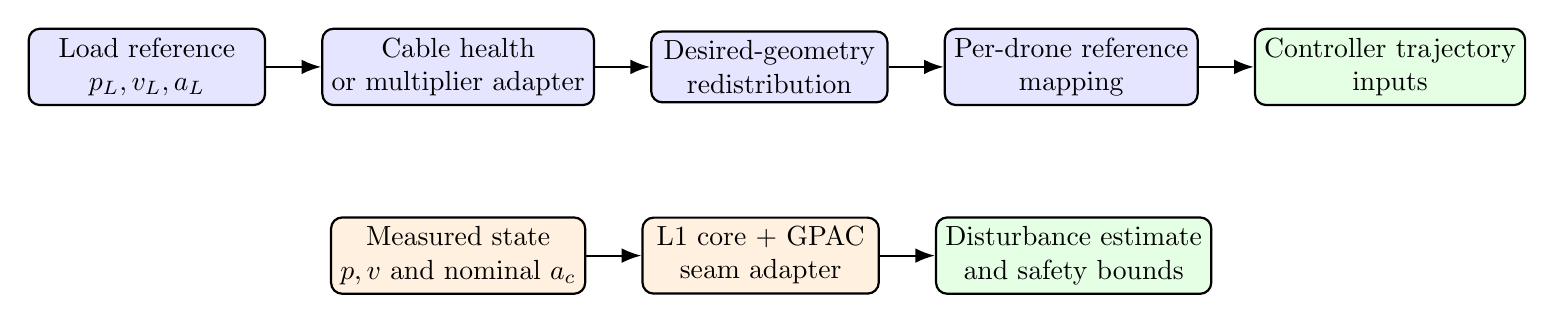
\begin{tikzpicture}[
  node distance=6mm and 7mm,
  block/.style={draw, rounded corners, thick, minimum width=3.0cm, minimum height=0.9cm, align=center},
  nominal/.style={block, fill=blue!10},
  adaptive/.style={block, fill=orange!12},
  result/.style={block, fill=green!10},
  arrow/.style={-{Latex[length=2.5mm]}, thick}
]
\node[nominal] (load) {Load reference\\$p_L,v_L,a_L$};
\node[nominal, right=of load] (health) {Cable health\\or multiplier adapter};
\node[nominal, right=of health] (redistribute) {Desired-geometry\\redistribution};
\node[nominal, right=of redistribute] (map) {Per-drone reference\\mapping};
\node[result, right=of map] (traj) {Controller trajectory\\inputs};

\node[adaptive, below=14mm of health] (state) {Measured state\\$p,v$ and nominal $a_c$};
\node[adaptive, right=of state] (l1) {L1 core + GPAC\\seam adapter};
\node[result, right=of l1] (dist) {Disturbance estimate\\and safety bounds};

\draw[arrow] (load) -- (health);
\draw[arrow] (health) -- (redistribute);
\draw[arrow] (redistribute) -- (map);
\draw[arrow] (map) -- (traj);
\draw[arrow] (state) -- (l1);
\draw[arrow] (l1) -- (dist);
\end{tikzpicture}
\caption{Fault-tolerant signal flow. PID-plus-feedforward control (Proposition~\ref{thm:topology_invariance}) with load-tracking integral on payload GPS closes the loop on actual payload position. Geometry redistribution (dashed) is implemented but not active in the reported runs.}
\label{fig:control_signal_flow}
\end{figure*}


\section{Experimental Methodology and Evidence Sources}\label{Section_V:Experimental_Methodology}
This paper distinguishes three levels of claim: \textit{implemented} modules that exist in the codebase, \textit{reproducible} results reproducible from canonical artifacts, and \textit{open} hypotheses whose formal proof is incomplete (see the evidence-level summary in Section~\ref{Section_IV:Fault-Tolerant_Control_Architecture}). The full-Drake simulations use the GPAC hierarchy's PID-plus-feedforward control law (Section~\ref{Section_IV:Fault-Tolerant_Control_Architecture}) with PID feedback, gravity feedforward, and cable-tension feedforward as the fault-tolerance mechanism. The ESO feedforward and adaptive estimation are disabled. The reduced-order comparisons retain the CL baseline as the standardized reference. The related code, including the full-Drake scenarios, experiment drivers, and analysis scripts used in this study, is available in the public Tether\_Grace repository~\cite{hajieghrary2026tethergrace}. That repository serves as the canonical source for the reproducible artifacts referenced throughout this section.

\subsection{Scenario Families and Evaluation Pipeline}

The primary full-Drake scenario families are:
\begin{enumerate}[label=(\alph*),nosep]
  \item canonical abrupt cable faults for $N \in \{3, 5, 7\}$;
  \item matched single-fault comparison across $N \in \{3, 5, 7\}$ with identical fault event (cable~$0$ at $t = 7.0$~s), deconfounding team size from fault count;
  \item cable-tension feedforward ablation ($\kappa_T \in \{0, 0.25, 0.5, 1.0\}$) in $N{=}3$;
  \item thrust saturation boundary sweep ($f_{\max} \in \{35, 38, 45, 60, 80, 150\}$~N) in $N{=}3$;
  \item controller comparison hierarchy including centralized oracle, reactive FTC, and gain-scheduled PID baselines;
  \item ESO-active evaluation to assess $\rho_{\mathrm{FT}}$ sensitivity to controller complexity;
  \item broadened Monte Carlo with randomized payload mass (${\pm}10\%$), PID gains (${\pm}10\%$), and fault timing (${\pm}2$~s);
  \item cable discretization sensitivity: bead count $n_b \in \{2, 4, 8, 12, 16\}$ in the $N{=}5$ cascading-fault scenario, holding cable-level stiffness and damping invariant to isolate the effect of spatial resolution on transient load dynamics.
\end{enumerate}
Complementary reduced-order studies---CL fidelity comparison, history-management diagnostics, gradual degradation, and non-CL adaptive law search---are reported in the supplementary material.

The primary metric is post-fault payload tracking RMSE, available across all standardized scenarios. For fidelity comparison, the key statistic is the full-Drake to reduced-order RMSE ratio under matched conditions. For history corruption, the main quantities are CL bias duration and stack refill time. For topology-margin screening, capacity and effective-capacity ratios are reported rather than closed-form proofs.

The evidence is organized in two tiers: (i)~ideal-condition runs (plant state, no wind) establishing the core mechanism and scalability, and (ii)~sensor-realistic runs (ESKF + Dryden wind) and Monte Carlo campaigns establishing robustness. Both tiers report RMSE and peak error ($\mathcal{L}_\infty$) to enable comparison with the theoretical bound (Proposition~\ref{thm:topology_invariance}).


\section{Simulation Results}\label{Section_VI:Simulation_Results}
This section reports full-Drake multibody simulation results across $N \in \{3, 5, 7\}$ with abrupt cable-snap faults. All results use the Drake~\cite{drake2024} plant at $\Delta t_{\mathrm{sim}} = 0.2$~ms with bead-chain cable dynamics and $30$~s figure-eight trajectories. Specifically, each physical cable is modeled as a chain of 8 point-mass beads connected by 9 tension-only spring-damper segments. This high-fidelity representation captures realistic elastic tension surges and slack behavior during abrupt severing faults, distinguishing it from the simplified scalar topology used for the analytical bounds.

\begin{remark}[System Under Test]\label{rem:system_under_test}
The full-Drake results use Layers~1--2 of the GPAC hierarchy (PID position control with gravity/cable-tension feedforward and geometric $\SOthree$ attitude control). Layer~3 (CL mass estimator), Layer~4 (ESO), and the $\mathcal{L}_1$ adaptive path are \textbf{disabled}. The CBF safety filter is \textbf{disabled}. Sensor state is \textbf{plant-state-direct} (ESKF disabled). Wind disturbance is \textbf{disabled} in the ideal runs; ESKF and Dryden wind are \textbf{active} in the sensor-realistic evaluation.
\end{remark}

The per-agent controller uses PID position feedback ($k_p = 8.0$, $k_d = 8.0$, $k_i = 0.15$), gravity feedforward, cable-tension feedforward ($\kappa_T = 0.5$), anti-swing damping ($k_{\mathrm{sw}} = 0.5$), and geometric $\SOthree$ attitude tracking---all N-agnostic by construction. Three canonical scenarios of increasing difficulty are evaluated:

\begin{enumerate}[label=(\roman*),nosep]
  \item \emph{Three drones, single fault:} $N = 3$, cable lengths $[1.00, 1.08, 1.16]$~m. Cable~$0$ severed at $t_f = 7.0$~s. Post-fault: $2$ agents, $50\%$ load-share increase.
  \item \emph{Five drones, two cascading faults:} $N = 5$, cable lengths $[1.00, 1.05, 1.10, 1.14, 1.18]$~m. Cable~$1$ at $7.0$~s, cable~$3$ at $12.0$~s. Post-fault: $3$ agents, $67\%$ increase.
  \item \emph{Seven drones, three cascading faults:} $N = 7$, cable lengths $[0.98, 1.01, 1.04, 1.07, 1.10, 1.13, 1.16]$~m. Cables~$1$, $3$, $5$ at $7.0$, $12.0$, $14.0$~s. Post-fault: $4$ agents, $75\%$ increase.
\end{enumerate}

No agent is informed of topology changes except the freed agent itself, which detects its own cable loss via $T_i < T_{\min}$.

% ============================================================
\subsection{Canonical Fault Scenarios}
\label{sec:payload_tracking}
% ============================================================

Table~\ref{tab:scenario_summary} reports payload tracking performance across all canonical scenarios. The ${\sim}35$~cm nominal RMSE reflects PID-only control by design; the full GPAC stack (CL+ESO) would reduce it but would introduce history-dependent terms breaking the topology-invariant structure. The favorable $\rho_{\mathrm{FT}}$ values ($1.26$--$1.39$) partly reflect this choice (larger denominator); with the full stack, $\rho_{\mathrm{FT}}$ increases modestly (Section~\ref{sec:eso_evaluation}). The absolute post-fault RMSE ($44$--$49$~cm) is the operationally relevant quantity: it is about three payload radii and roughly $40\%$ of a nominal $1.0$--$1.2$~m cable length, so the controller preserves transport continuity rather than precision placement. Empirical $\rho_{\mathrm{FT}}^{\mathrm{emp}}$ falls below the conservative bound $N/(N{-}k)$ from~\eqref{eq:rho_closed_form}, consistent with the transient-aware analysis in Section~\ref{sec:topology_invariance_theorem}. The canonical scenarios themselves confound team size with fault count; the matched single-fault comparison below isolates the team-size effect.

\begin{table}[t]
\centering
\caption{Full-Drake payload tracking performance: nominal and fault scenarios.}
\label{tab:scenario_summary}
\begin{tabular}{lcccc}
\toprule
Scenario & $N$ & Load RMSE & Peak error & $\rho_{\mathrm{FT}}^{\mathrm{emp}}$ \\
         &     & [cm]      & [cm]       &  \\
\midrule
Three drones, no fault  & 3 & 35.12 & 110.57 & --- \\
Five drones, no fault   & 5 & 34.84 & 110.10 & --- \\
Seven drones, no fault  & 7 & 34.70 & 108.65 & --- \\
\midrule
Three drones, 1~fault   & 3 & 48.84 & 107.44 & 1.39 \\
Five drones, 2~faults   & 5 & 46.37 & 112.30 & 1.33 \\
Seven drones, 3~faults  & 7 & 43.60 & 117.45 & 1.26 \\
\bottomrule
\end{tabular}
\end{table}

The canonical scenarios suggest that average payload RMSE falls with team size even while the number of faults increases: the $N{=}7$ scenario absorbs three cascading faults yet achieves $11\%$ lower RMSE than $N{=}3$ with one fault. Peak errors ($107$--$117$~cm) settle within $1$--$2$~s (Figs.~\ref{fig:tracking_errors_all},~\ref{fig:load_error_overlay}), and each snap produces a bounded reconfiguration rather than loss of transport (Fig.~\ref{fig:scenario_seven}). The matched single-fault comparison below shows that the same trend persists once the fault schedule is held fixed.

\begin{figure*}

    \centering
    \begin{subfigure}[t]{0.24\textwidth}
    \centering
    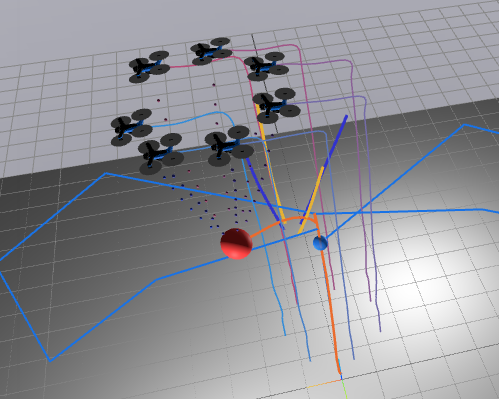
\includegraphics[width=\textwidth]{./Figures/full_drake/seven_drones/7-drones_0.png}
    \caption{}
    \end{subfigure}
    \hfill
    \begin{subfigure}[t]{0.24\textwidth}
    \centering
      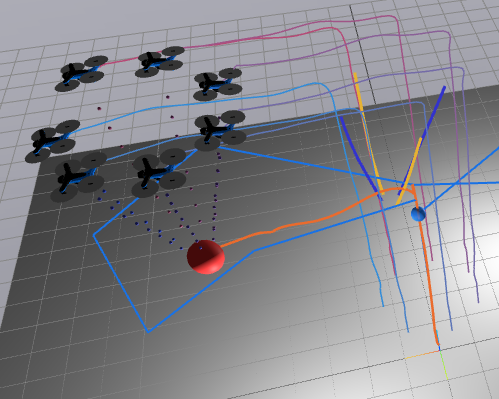
\includegraphics[width=\textwidth]{./Figures/full_drake/seven_drones/7-drones_1.png}
      \caption{}
    \end{subfigure}
    \hfill
    \begin{subfigure}[t]{0.24\textwidth}
    \centering
      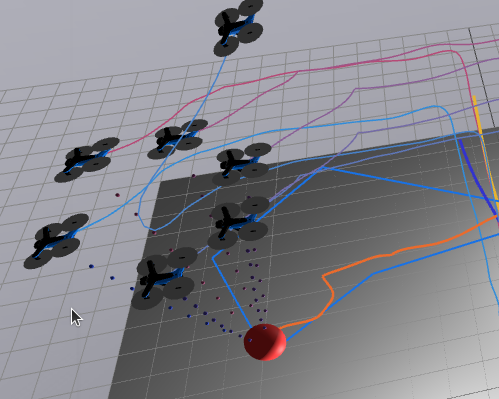
\includegraphics[width=\textwidth]{./Figures/full_drake/seven_drones/7-drones_2.png}
      \caption{}
    \end{subfigure}
    \begin{subfigure}[t]{0.24\textwidth}
    \centering
      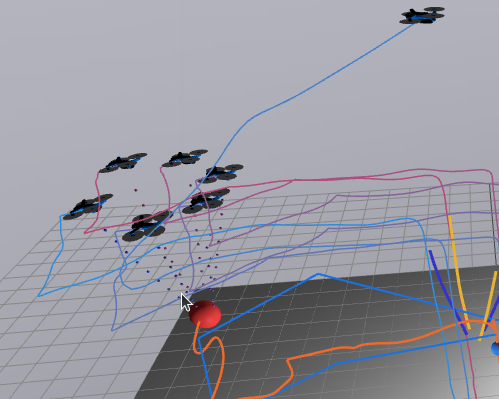
\includegraphics[width=\textwidth]{./Figures/full_drake/seven_drones/7-drones_3.png}
      \caption{}
    \end{subfigure}

     \vspace{0.5em} % Space between rows

     % Row 2
     \begin{subfigure}[b]{0.24\textwidth}
        \centering
        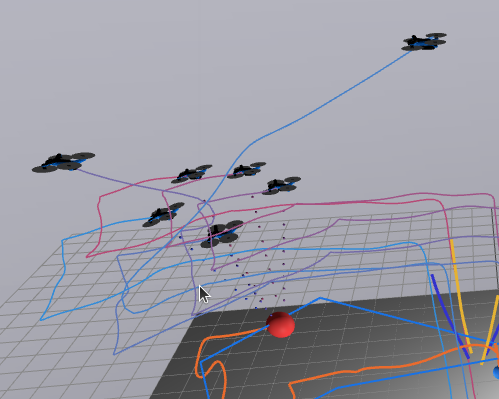
\includegraphics[width=\textwidth]{./Figures/full_drake/seven_drones/7-drones_4.png}
        \caption{}
     \end{subfigure}
     \hfill
      \begin{subfigure}[b]{0.24\textwidth}
        \centering
        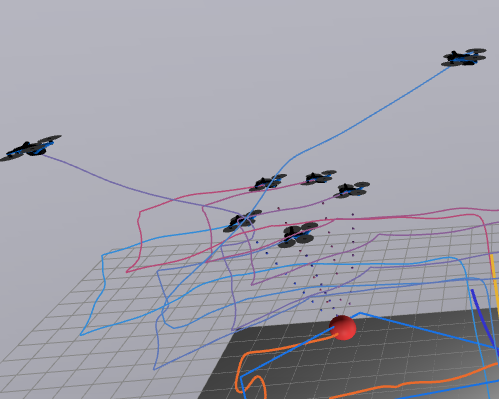
\includegraphics[width=\textwidth]{./Figures/full_drake/seven_drones/7-drones_5.png}
        \caption{}
     \end{subfigure}
      \begin{subfigure}[b]{0.24\textwidth}
        \centering
        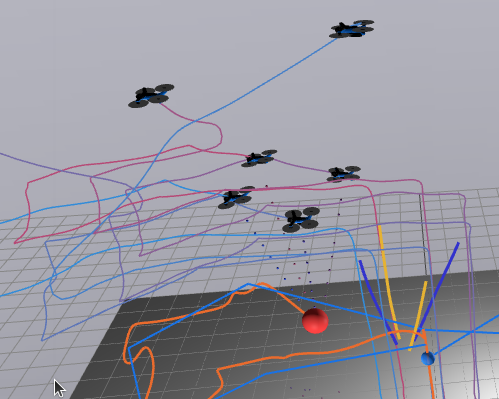
\includegraphics[width=\textwidth]{./Figures/full_drake/seven_drones/7-drones_6.png}
        \caption{}
     \end{subfigure}
      \begin{subfigure}[b]{0.24\textwidth}
        \centering
        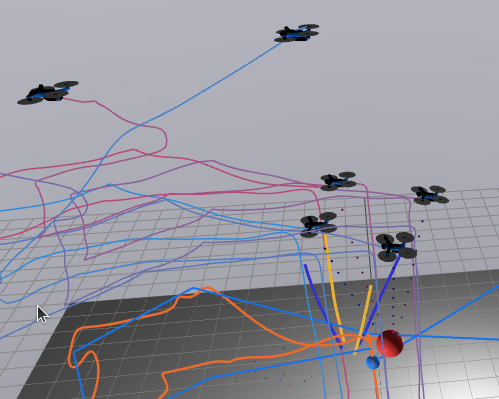
\includegraphics[width=\textwidth]{./Figures/full_drake/seven_drones/7-drones_7.png}
        \caption{}
     \end{subfigure}

  \caption{Seven-drone scenario ($N = 7$, cables~$1$, $3$, $5$ at $7.0$, $12.0$, $14.0$~s). (a) at the start of the mission. (b) about $1$~s before first fault. (c) about  $1$~s after first fault. (d) about $1$~s before second fault. (e) about $1$~s after second fault. (f) about $1$~s before third fault. (g) about $1$~s after third fault. (h) Settled after all faults: $Q_0$, $Q_2$, $Q_4$, $Q_6$ remain.}
  \label{fig:scenario_seven}
\end{figure*}

Cable tensions (Fig.~\ref{fig:tensions_all}) confirm the load-redistribution mechanism: when a cable snaps, remaining cables exhibit a tension surge as they absorb the redistributed load. The freed agent detects the fault via $T_i < T_{\min}$ within the $0.12$~s debounce window and initiates escape. Detection latency is consistent across all six fault events (Table~\ref{tab:fault_detection}), with all freed agents reaching $2.06$--$4.73$~m final separation. Progressive tension oscillation growth reflects cable pendulum near-resonance (${\sim}2$~s period vs.\ ${\sim}3$~s trajectory corner interval); all tensions remain positive, with peaks (${\sim}25$~N) well within limits ($f_{\max} = 150$~N).

\begin{figure}[t]
\centering
\begin{subfigure}[t]{\columnwidth}
  \centering
  
\includegraphics[width=\columnwidth]{./Figures/full_drake/three_drones/payload_tracking_error.png}
  \caption{$N = 3$, single fault at $t = 7.0$~s.}
  \label{fig:tracking_error_three}
\end{subfigure}\\[2pt]
\begin{subfigure}[t]{\columnwidth}
  \centering
  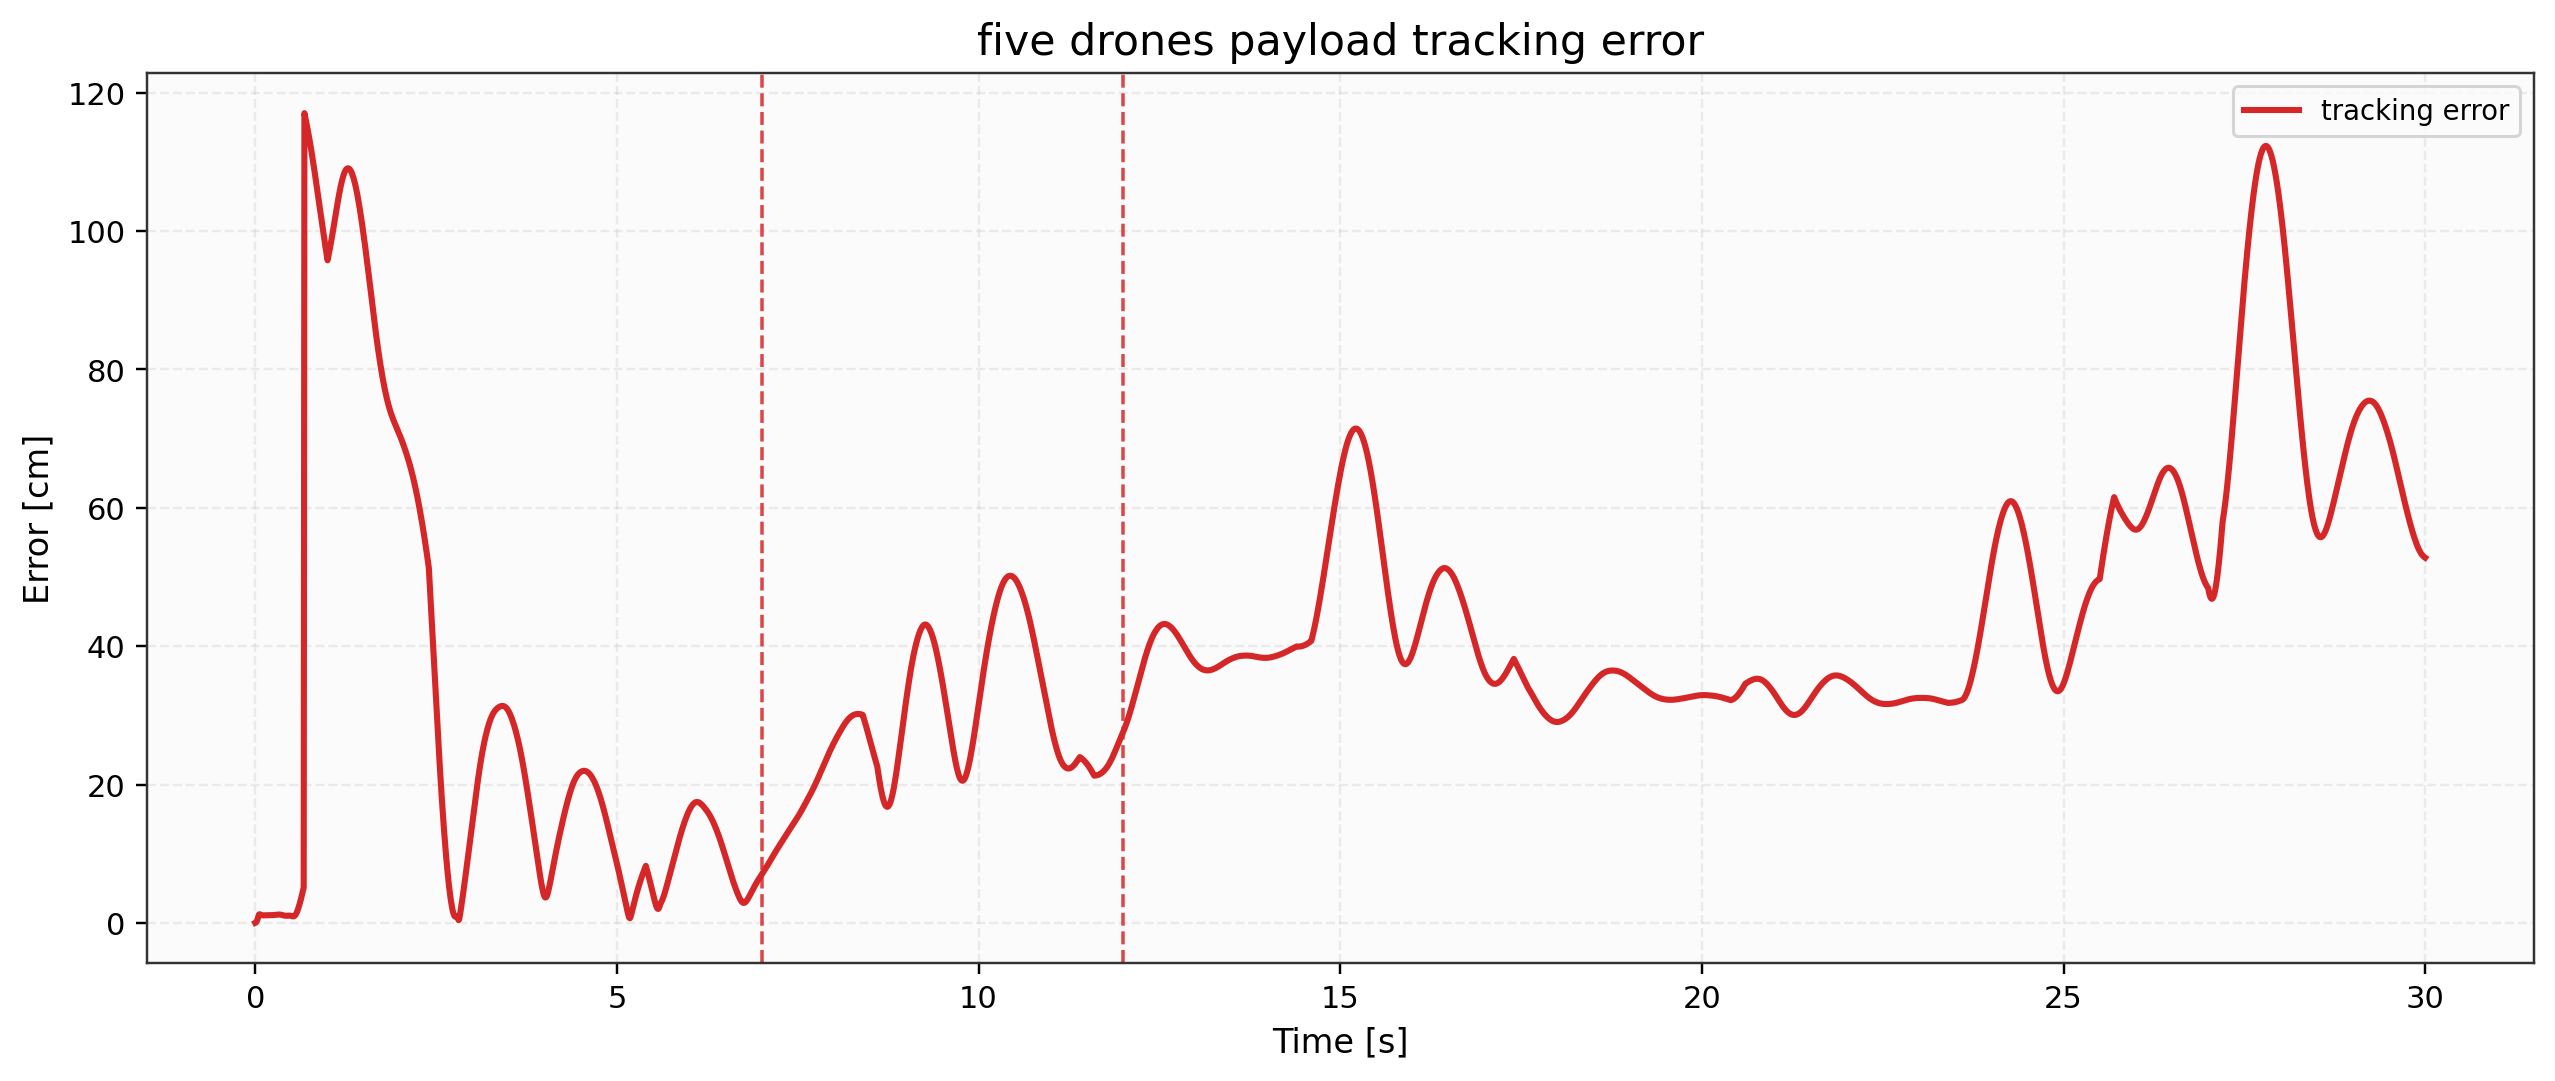
\includegraphics[width=\columnwidth]{./Figures/full_drake/five_drones/payload_tracking_error.png}
  \caption{$N = 5$, two cascading faults.}
  \label{fig:tracking_error_five}
\end{subfigure}\\[2pt]
\begin{subfigure}[t]{\columnwidth}
  \centering
  
\includegraphics[width=\columnwidth]{./Figures/full_drake/seven_drones/payload_tracking_error.png}
  \caption{$N = 7$, three cascading faults within $7$~s.}
  \label{fig:tracking_error_seven}
\end{subfigure}
\caption{Payload tracking error across scenarios. Each fault produces a bounded transient settling in $1$--$2$~s without explicit fault handling.}
\label{fig:tracking_errors_all}
\end{figure}

\begin{figure}[t]
\centering
\begin{subfigure}[t]{\columnwidth}
  \centering
  
\includegraphics[width=\columnwidth]{./Figures/full_drake/three_drones/cable_tensions.png}
  \caption{$N = 3$. Cable~$0$ snaps at $t = 7.0$~s; cables~$1$, $2$ absorb the load.}
  \label{fig:tensions_three}
\end{subfigure}\\[2pt]
\begin{subfigure}[t]{\columnwidth}
  \centering
  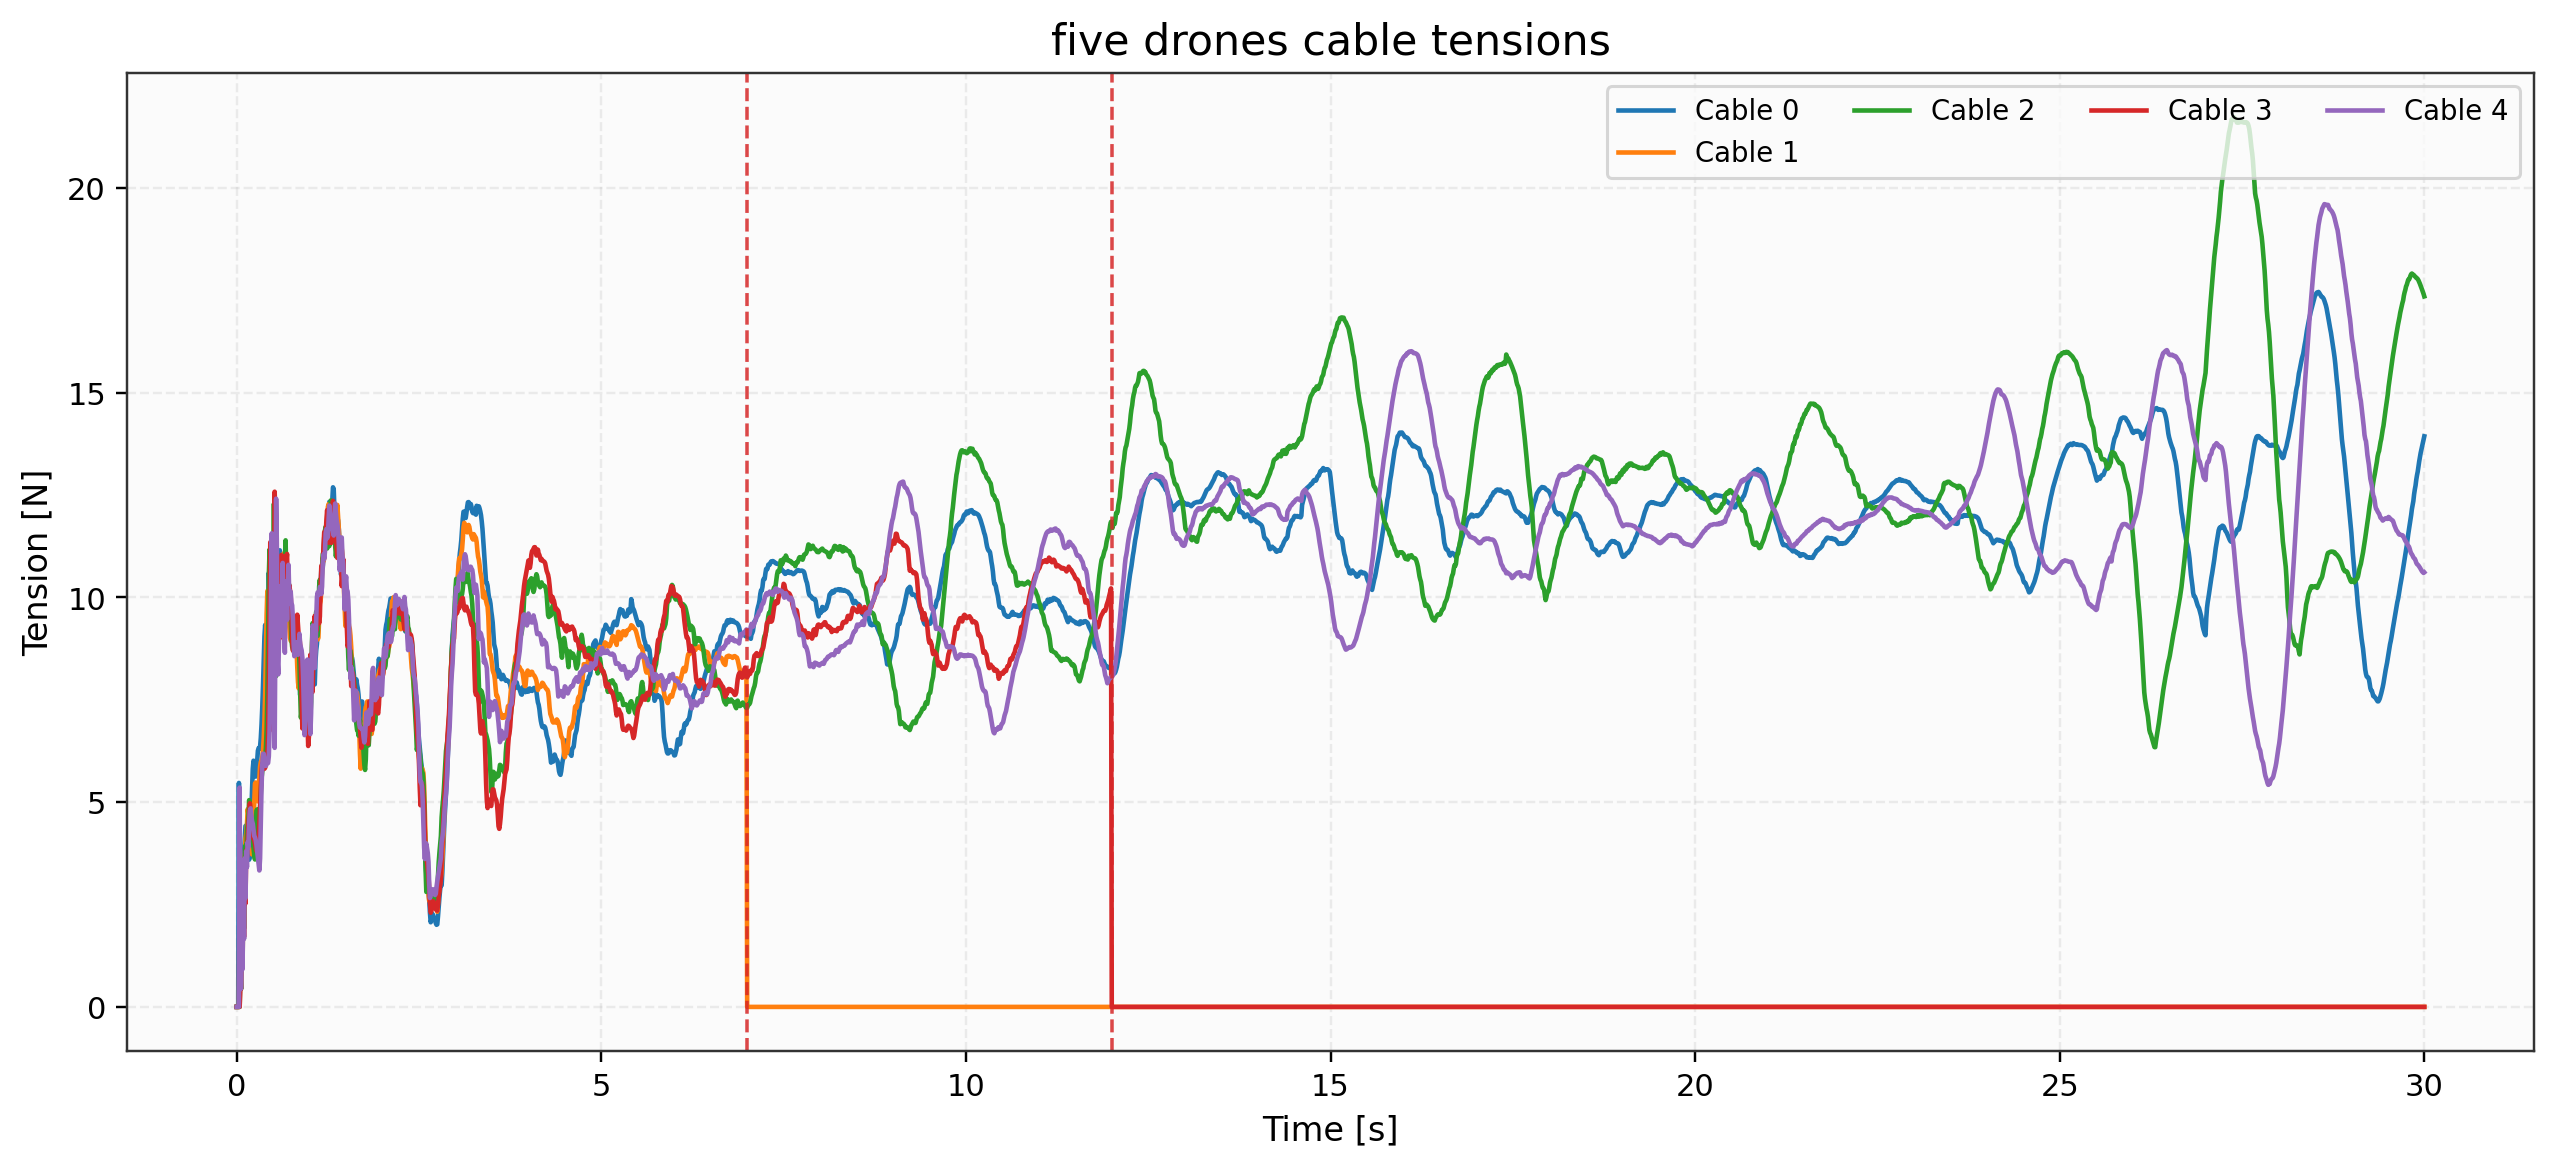
\includegraphics[width=\columnwidth]{./Figures/full_drake/five_drones/cable_tensions.png}
  \caption{$N = 5$. Sequential faults at $7.0$~s and $12.0$~s.}
  \label{fig:tensions_five}
\end{subfigure}\\[2pt]
\begin{subfigure}[t]{\columnwidth}
  \centering
  
\includegraphics[width=\columnwidth]{./Figures/full_drake/seven_drones/cable_tensions.png}
  \caption{$N = 7$. Three sequential faults; four surviving cables remain within limits.}
  \label{fig:tensions_seven}
\end{subfigure}
\caption{Cable tension dynamics across scenarios. Remaining cables exhibit tension surges upon load redistribution; all tensions remain positive and within limits.}
\label{fig:tensions_all}
\end{figure}

\begin{table}[t]
\centering
\caption{Fault detection and freed-agent separation.}
\label{tab:fault_detection}
\begin{tabular}{lcccccc}
\toprule
Scen. & Drone & $t_f$ & Detect. & \multicolumn{3}{c}{Healthy separation [m]} \\
      &       & [s]   & [s]     & at fault & +2\,s & final \\
\midrule
$N{=}3$ & 0 & 7.0  & 0.12 & 0.90 & 1.27 & 2.26 \\
\midrule
$N{=}5$ & 1 & 7.0  & 0.12 & 0.66 & 1.07 & 2.69 \\
        & 3 & 12.0 & 0.12 & 0.65 & 1.96 & 4.68 \\
\midrule
$N{=}7$ & 1 & 7.0  & 0.12 & 0.50 & 1.05 & 2.06 \\
        & 3 & 12.0 & 0.12 & 0.50 & 1.90 & 4.73 \\
        & 5 & 14.0 & 0.12 & 0.50 & 1.69 & 3.82 \\
\bottomrule
\end{tabular}
\end{table}

Vehicle-level dynamics for the most demanding case ($N{=}7$, Fig.~\ref{fig:vehicle_dynamics_seven}) confirm that the GPAC hierarchy maintains stability throughout: after cascading faults, drones~$1$, $3$, $5$ escape while drones~$0$, $2$, $4$, $6$ continue tracking. Formation deviation shows bounded steps at each fault, tilt stays within safe limits, and peak thrust (${\sim}40$~N) remains well below $f_{\max} = 150$~N. The cross-scenario overlay (Fig.~\ref{fig:load_error_overlay}) confirms comparable pre-fault tracking across team sizes, localized $40$--$60$~cm transients per fault event, and stable control even in the $N{=}7$ stress test where the third fault occurs before full recovery from the second. While run-averaged RMSE improves with $N$, terminal error at $t = 30$~s is $42.36$, $52.79$, $54.62$~cm---larger teams improve average tracking but the multi-fault schedules do not produce the smallest end-of-run residual.

\begin{figure*}[t]
\centering
\begin{subfigure}[t]{0.48\textwidth}
  \centering
  
\includegraphics[width=\textwidth]{./Figures/full_drake/seven_drones/xy_trajectories.png}
  \caption{XY trajectories. Drones~$1$, $3$, $5$ depart; $0$, $2$, $4$, $6$ continue.}
  \label{fig:xy_traj_seven}
\end{subfigure}\hfill
\begin{subfigure}[t]{0.48\textwidth}
  \centering
  
\includegraphics[width=\textwidth]{./Figures/full_drake/seven_drones/quad_formation_deviation.png}
  \caption{Formation deviation. Each fault produces a bounded step.}
  \label{fig:formation_seven}
\end{subfigure}\\[4pt]
\begin{subfigure}[t]{0.48\textwidth}
  \centering
  
\includegraphics[width=\textwidth]{./Figures/full_drake/seven_drones/quad_tilt_magnitude.png}
  \caption{Vehicle tilt. Remains within safe limits through all fault transients.}
  \label{fig:tilt_seven}
\end{subfigure}\hfill
\begin{subfigure}[t]{0.48\textwidth}
  \centering
  
\includegraphics[width=\textwidth]{./Figures/full_drake/seven_drones/quad_force_norm.png}
  \caption{Thrust per vehicle. Post-fault ${\sim}40$~N, well below $f_{\max} = 150$~N.}
  \label{fig:force_seven}
\end{subfigure}
\caption{Vehicle-level dynamics for $N = 7$ with three cascading faults. The GPAC hierarchy maintains stability: tilt stays within safe limits and thrust remains well below saturation.}
\label{fig:vehicle_dynamics_seven}
\end{figure*}

\begin{figure}[t]
\centering
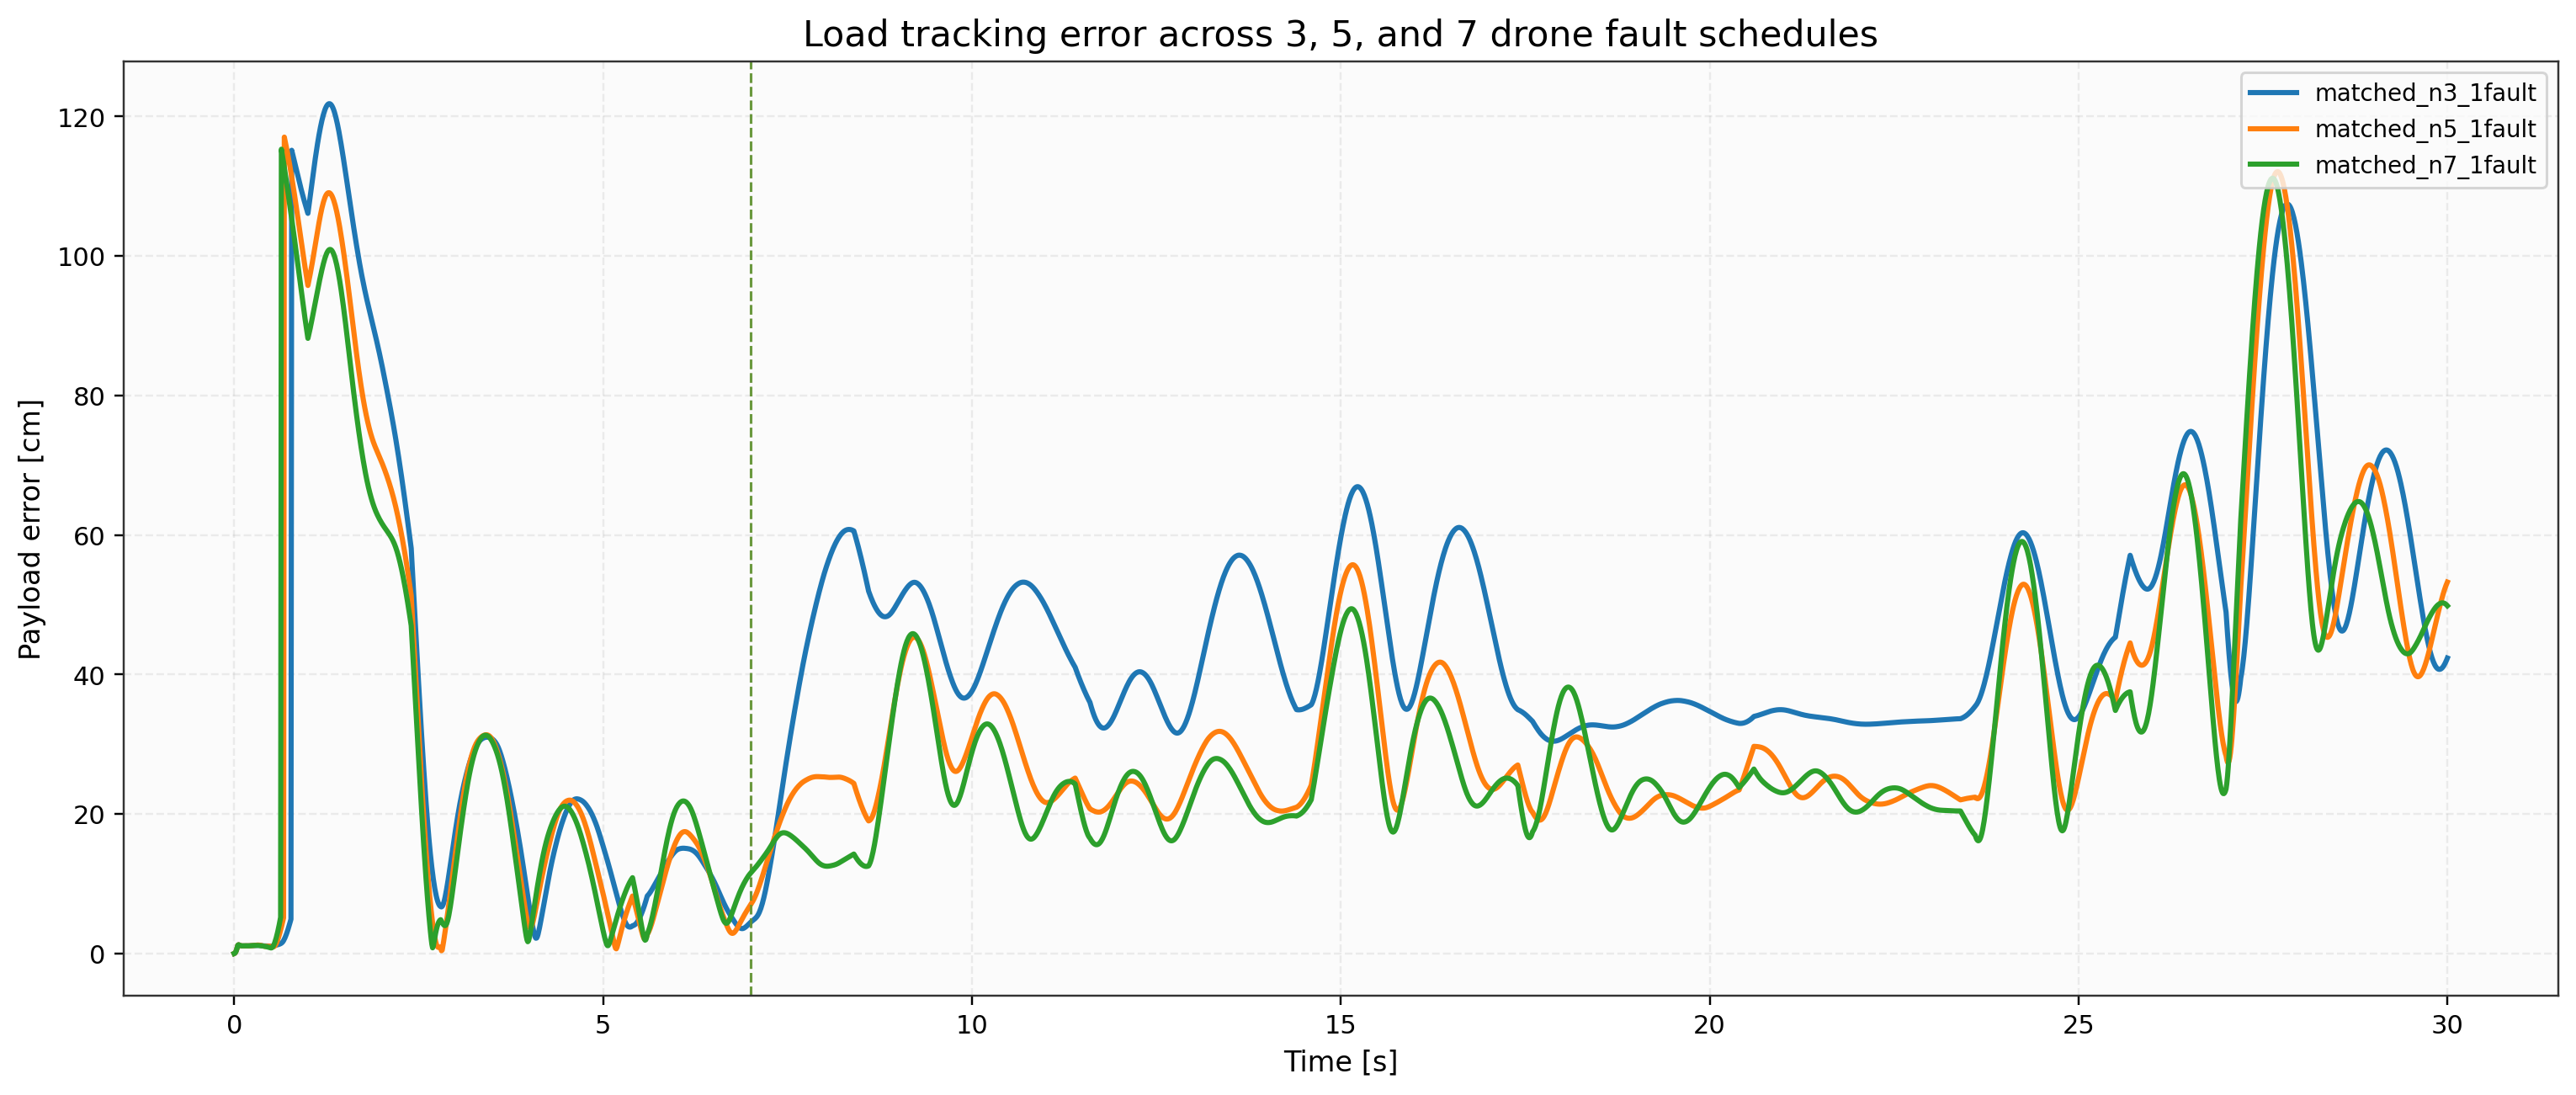
\includegraphics[width=\columnwidth]{./Figures/full_drake/batch_comparison/comparison_load_error_overlay.png}
\caption{Payload tracking error overlay across $N = 3$, $5$, $7$. Fault responses remain localized, settling on $1$--$2$~s timescales.}
\label{fig:load_error_overlay}
\end{figure}

% ============================================================
\subsection{Deconfounding by Team Size, Fault Count, and Thrust Margin}
\label{sec:matched_single_fault}
% ============================================================

The canonical scenarios confound team size with fault count ($1$, $2$, $3$ faults for $N = 3, 5, 7$). Two complementary experiments isolate these variables.

\emph{Matched single-fault comparison.}\label{sec:matched_single_fault_exp}
Applying the \emph{same single-fault event} (cable~$0$ at $t = 7.0$~s) across all three team sizes (Table~\ref{tab:matched_single_fault}), RMSE decreases monotonically: $48.84 \to 40.37 \to 38.38$~cm ($21\%$ improvement from $N{=}3$ to $N{=}7$), confirming that larger capacity ratios translate directly to better tracking. Peak error is nearly constant (${\sim}107$--$112$~cm), set by the cable-snap impulse magnitude. The RMSE improvement comes from faster mid-trajectory recovery, not better final convergence ($N{=}3$ achieves the lowest terminal residual at $42.36$~cm).

\begin{table}[t]
\centering
\caption{Matched single-fault comparison: identical fault event across team sizes.}
\label{tab:matched_single_fault}
\begin{tabular}{lcccc}
\toprule
& $N{=}3$ & $N{=}5$ & $N{=}7$ \\
\midrule
Post-fault capacity ratio & $2/3$ & $4/5$ & $6/7$ \\
Load RMSE [cm]           & 48.84 & 40.37 & 38.38 \\
Peak error [cm]          & 107.44 & 112.09 & 111.15 \\
Final error [cm]         & 42.36 & 53.25 & 49.85 \\
\bottomrule
\end{tabular}
\end{table}

\emph{Fault-count isolation.}\label{sec:fault_count_isolation}
Holding $N{=}7$ constant while varying $k \in \{1, 2, 3\}$ (Table~\ref{tab:fault_count_isolation}), RMSE increases monotonically: $34.70$, $39.39$, $41.29$, $43.60$~cm for $k = 0, 1, 2, 3$. Each additional fault adds ${\sim}2$--$5$~cm RMSE, confirming incremental degradation rather than catastrophic failure. Peak error is highest for $k{=}2$ ($118.21$~cm), likely because the second fault at $t{=}12$~s occurs during an unfavorable trajectory phase.

\begin{table}[t]
\centering
\caption{Fault-count isolation: $N{=}7$ with 1, 2, and 3 faults.}
\label{tab:fault_count_isolation}
\begin{tabular}{lccccc}
\toprule
Faults $k$ & Surviving & Capacity & RMSE & Peak & Final \\
           & agents    & ratio    & [cm] & [cm] & [cm]  \\
\midrule
0 (nominal) & 7 & --- & 34.70 & 108.65 & 43.73 \\
1           & 6 & $6/7$ & 39.39 & 111.26 & 54.43 \\
2           & 5 & $5/7$ & 41.29 & 118.21 & 54.74 \\
3           & 4 & $4/7$ & 43.60 & 117.45 & 54.62 \\
\bottomrule
\end{tabular}
\end{table}

\emph{Thrust-margin verification.}
All scenarios satisfy the thrust-margin condition with capacity ratios $1.75$--$2.33$ (Table~\ref{tab:topology_margin}). Peak tilt during post-fault transients ($15$\textdegree--$25$\textdegree, Fig.~\ref{fig:tilt_seven}) reduces effective vertical thrust by $3$--$9\%$; all scenarios remain well above unity with this correction. A conservative design should use $f_{\max} \cos(\theta_{\max})$ as the effective vertical thrust authority.

\begin{table}[t]
\centering
\caption{Topology-invariance thrust-margin screen.}
\label{tab:topology_margin}
\begin{tabular}{lccccc}
\toprule
Scenario & $N$ & Required & Available & Capacity & Healthy \\
         &     & [N/agent]& [N/agent] & ratio    & fraction \\
\midrule
$N{=}3$, 1~fault & 3 & 29.43 & 51.50 & 1.75 & 0.67 \\
$N{=}5$, 2~faults & 5 & 24.53 & 51.50 & 2.10 & 0.60 \\
$N{=}7$, 3~faults & 7 & 22.07 & 51.50 & 2.33 & 0.57 \\
\bottomrule
\end{tabular}
\end{table}

% ============================================================
\subsection{Mechanism Identification}
\label{sec:tension_ablation}
% ============================================================

Three experiments identify what drives the fault-absorption mechanism and where it breaks.

\emph{Tension feedforward ablation.}\label{sec:fmax_boundary}
Disabling cable-tension feedforward in the most stressed scenario ($N{=}3$, single fault) changes RMSE by only $0.44$~cm ($0.9\%$) and peak error by $0.06$~cm (Table~\ref{tab:tension_ablation}). Varying $\kappa_T$ across $\{0, 0.25, 0.5, 1.0\}$ produces total RMSE variation of $1.55$~cm. This identifies the \emph{primary} fault-absorption mechanism as PID feedback with gravity feedforward---not cable-tension feedforward. Cable-tension feedforward provides a marginal improvement ($0.77$~cm in final error) that is helpful but not essential.

\begin{table}[t]
\centering
\caption{Tension feedforward ablation ($N{=}3$, single fault at $t = 7.0$~s).}
\label{tab:tension_ablation}
\begin{tabular}{lccc}
\toprule
Configuration & RMSE [cm] & Peak [cm] & Final [cm] \\
\midrule
Full feedforward ($\kappa_T = 0.5$) & 48.84 & 107.44 & 42.36 \\
No tension feedforward              & 48.40 & 107.50 & 43.13 \\
\bottomrule
\end{tabular}
\end{table}

\emph{Thrust saturation boundary.}
Sweeping $f_{\max}$ from $150$~N down to $35$~N reveals a sharp phase transition (Table~\ref{tab:fmax_boundary}): for $f_{\max} \in [45, 150]$~N, RMSE stays within $48.8$--$49.1$~cm; at $f_{\max} = 38$~N, it jumps to $236.9$~cm ($4.9\times$ degradation). This coincides with the theoretical minimum:
\begin{equation}\label{eq:fmax_critical}
  f_{\max}^* = \frac{(N \cdot m_Q + m_L) \cdot g}{N - k} + f_{\mathrm{track}} \approx 36.8 + 8 \approx 45\;\text{N},
\end{equation}
where $f_{\mathrm{track}} \approx m_Q \cdot a_{\max} \approx 8$~N accounts for figure-eight tracking demand (matching the observed pre-fault thrust above hover). The default $f_{\max} = 150$~N provides $3\times$ headroom, confirming that the claimed fault tolerance does not depend on aggressive actuator sizing. Below the transition, RMSE is non-monotonic ($236.9$~cm at $38$~N vs.\ $192.1$~cm at $35$~N): the system enters distinct saturation-dominated failure modes where the specific trajectory phase at the fault instant determines which agents saturate and for how long.

\begin{table}[t]
\centering
\caption{Thrust saturation boundary ($N{=}3$, single fault at $t = 7.0$~s).}
\label{tab:fmax_boundary}
\begin{tabular}{lcccc}
\toprule
$f_{\max}$ [N] & $f_{\max}/f_{\mathrm{hover}}$ & RMSE [cm] & Peak [cm] & Final [cm] \\
\midrule
150 & $10.2\times$ & 48.84 & 107.44 & 42.36 \\
 80 & $ 5.4\times$ & 48.84 & 107.44 & 42.36 \\
 60 & $ 4.1\times$ & 48.84 & 107.44 & 42.36 \\
 45 & $ 3.1\times$ & 49.06 & 107.66 & 44.10 \\
 38 & $ 2.6\times$ & 236.92 & 324.97 & 252.35 \\
 35 & $ 2.4\times$ & 192.11 & 250.34 & 179.28 \\
\bottomrule
\end{tabular}
\end{table}

\emph{Controller comparison hierarchy.}\label{sec:baseline_comparison}
To contextualize the passive GPAC approach, three alternative controllers are evaluated on the $N{=}3$ single-fault scenario (Table~\ref{tab:baseline_comparison}): a centralized oracle with perfect post-fault load-share feedforward, a gain-scheduled PID triggered by elevated cable tension, and a threshold-triggered reactive controller that boosts thrust by $+30\%$. The centralized oracle performs comparably to passive GPAC ($49.18$ vs.\ $48.84$~cm, $+0.7\%$), but this should be interpreted narrowly: the oracle only replaces the local cable-tension feedforward term and does not reconfigure geometry, reset the integral state, or alter the trajectory. The absolute difference is $0.34$~cm, smaller than the $0.49$~cm run-to-run standard deviation reported for the same $N{=}3$ fault scenario in Table~\ref{tab:monte_carlo}. The tested detection-based alternatives therefore provide no practically meaningful benefit over the N-agnostic PID-plus-feedforward structure, but this comparison does not rule out stronger centralized policies.

\begin{table}[t]
\centering
\caption{Controller comparison ($N{=}3$, single fault). The centralized oracle uses perfect post-fault load-share feedforward only; it does not alter geometry, trajectory references, or integral states.}
\label{tab:baseline_comparison}
\begin{tabular}{l S[table-format=2.2] S[table-format=3.2] l l}
\toprule
Controller & {RMSE} & {Peak} & Detection & Communication \\
           & [cm] & [cm]       &           &     \\
\midrule
Centralized oracle           & 49.18 & 107.33 & Perfect   & Yes \\
\midrule
Gain-scheduled PID & 48.96 & 106.75 & Threshold & No  \\
($1.5{\times}k_p, 1.25{\times}k_d$) &       &        &           &     \\
\midrule
\textbf{Passive GPAC}     & 48.84 & 107.44 & No        & No  \\
\midrule
Threshold-triggered  & 49.45 & 107.66 & Threshold & No  \\
\bottomrule
\end{tabular}
\end{table}

\emph{ESO-active evaluation.}\label{sec:eso_evaluation}
To assess whether the favorable $\rho_{\mathrm{FT}}$ values are an artifact of the deliberately constrained controller, the ESO disturbance feedforward (Layer~4) is activated in all canonical scenarios (Table~\ref{tab:eso_evaluation}). ESO reduces nominal RMSE by $17$--$18\%$, confirming that PID-only nominal RMSE was inflated by uncompensated cable dynamics. The $\rho_{\mathrm{FT}}$ values increase modestly ($1.37$--$1.46$ vs.\ $1.26$--$1.39$), but absolute post-fault RMSE with ESO ($40$--$46$~cm) is \emph{lower} than PID-only ($44$--$49$~cm)---the $\rho_{\mathrm{FT}}$ increase reflects proportionally larger nominal improvement, not degraded fault tolerance. The topology-invariance property does not hold strictly with ESO active (history dependence); the PID-only evaluation remains the correct test.

\begin{table}[t]
\centering
\caption{ESO-active evaluation: sensitivity of $\rho_{\mathrm{FT}}$ to controller complexity.}
\label{tab:eso_evaluation}
\begin{tabular}{lccccc}
\toprule
& \multicolumn{2}{c}{RMSE [cm]} & \multicolumn{2}{c}{$\rho_{\mathrm{FT}}$} \\
Scenario & Nominal & Fault & ESO & PID-only \\
\midrule
$N{=}3$, 1~fault & 28.94 & 40.43 & 1.40 & 1.39 \\
$N{=}5$, 2~faults & 30.50 & 44.59 & 1.46 & 1.33 \\
$N{=}7$, 3~faults & 33.67 & 46.01 & 1.37 & 1.26 \\
\bottomrule
\end{tabular}
\end{table}

% ============================================================
\subsection{Robustness Validation}
\label{sec:sensor_realistic}
% ============================================================

Four complementary evaluations establish robustness beyond the ideal-condition canonical runs.

\emph{Sensor-realistic evaluation.}
Activating the ESKF and Dryden wind model produces moderate, consistent RMSE degradation: $+9.9\%$ for $N{=}3$, $+8.1\%$ for $N{=}5$, and $+10.7\%$ for $N{=}7$ (Table~\ref{tab:sensor_realistic}). All scenarios remain stable with RMSE below $54$~cm, and the uniform ${\sim}10\%$ degradation confirms robustness to sensor noise and wind perturbations. Peak errors increase by $12$--$14$~cm, attributable to wind compounding fault transients and ESKF estimation lag.

\begin{table}[h]
\centering
\caption{Sensor-realistic evaluation}
\label{tab:sensor_realistic}
\begin{tabular}{lccccc}
\toprule
Scenario & \multicolumn{2}{c}{RMSE [cm]} & \multicolumn{2}{c}{Peak error [cm]} \\
         & Ideal & ESKF+wind & Ideal & ESKF+wind \\
\midrule
$N{=}3$, 1~fault   & 48.84 & 53.68 & 107.44 & 119.14 \\
$N{=}5$, 2~faults  & 46.37 & 50.14 & 112.30 & 125.17 \\
$N{=}7$, 3~faults  & 43.60 & 48.28 & 117.45 & 131.56 \\
\bottomrule
\end{tabular}
\end{table}

\emph{Monte Carlo validation.}\label{sec:monte_carlo}
A campaign of $N_{\mathrm{MC}} = 30$ runs per scenario randomizes cable lengths (${\pm}5\%$), wind seeds, and simulation seeds while using the same fixed fault schedule. Standard deviations of $0.49$--$1.34$~cm (Table~\ref{tab:monte_carlo}) confirm robustness to plant-parameter variation ($<3\%$ RMSE variation across $30$ runs). MC means are consistent with the deterministic values in Table~\ref{tab:scenario_summary} (within $1\%$), confirming representativeness. The 95th-percentile peak errors ($108$--$120$~cm) remain well within thrust-margin headroom.

\begin{table}[t]
\centering
\caption{Monte Carlo results (mean $\pm$ std over $N_{\mathrm{MC}}$ runs).}
\label{tab:monte_carlo}
\begingroup
\setlength{\tabcolsep}{3.5pt}
\renewcommand{\arraystretch}{0.96}
\footnotesize
\begin{tabular}{@{}lcccc@{}}
\toprule
Scenario & $N_{\mathrm{MC}}$ & RMSE [cm] & Peak [cm] & 95th pctl. \\
         &                    & mean $\pm$ std & mean $\pm$ std & peak [cm] \\
\midrule
$N{=}3$, 1 fault   & 30 & $48.84 \pm 0.49$ & $107.28 \pm 0.47$ & 107.85 \\
$N{=}5$, 2 faults  & 30 & $46.40 \pm 0.49$ & $112.23 \pm 1.07$ & 113.89 \\
$N{=}7$, 3 faults  & 30 & $43.95 \pm 1.34$ & $117.55 \pm 1.37$ & 119.84 \\
$N{=}3$, ESKF+wind & 30 & $53.62 \pm 0.83$ & $118.83 \pm 0.91$ & 120.19 \\
\bottomrule
\end{tabular}
\endgroup
\end{table}

\emph{Broadened Monte Carlo.}\label{sec:broadened_mc}
A broadened campaign additionally randomizes payload mass (${\pm}10\%$), PID gains (${\pm}10\%$), and fault timing (${\pm}2$~s). In $5$ runs for $N{=}3$, broadened RMSE is $48.04 \pm 1.29$~cm (vs.\ narrow MC $48.84 \pm 0.49$~cm): standard deviation increases ${\sim}2.6\times$ but all runs remain stable. Because this broadened campaign contains only five trials, it is interpreted here as exploratory evidence of robustness to simultaneous plant-parameter variation rather than as the same statistical tier as Table~\ref{tab:monte_carlo}.

\emph{Trajectory generalization.}\label{sec:trajectory_generalization}
Testing across hover, point-to-point, and figure-eight references in the supplementary material confirms that the fault-absorption mechanism operates consistently: RMSE decreases with team size and remains bounded across all trajectory types. Hover RMSE is $19\%$ lower than figure-eight ($39.75$ vs.\ $48.84$~cm for $N{=}3$), confirming that the figure-eight amplifies post-fault error through cable-pendulum near-resonance.

% ============================================================
\subsection{Cable Discretization Sensitivity}
\label{sec:bead_discretization}
% ============================================================

The bead-chain cable model discretizes each continuous cable into $n_b$ point-mass beads connected by $(n_b{+}1)$ tension-only spring-damper segments. All preceding results use $n_b{=}8$. A dedicated sweep over $n_b \in \{2, 4, 8, 12, 16\}$ in the $N{=}5$ cascading-fault scenario kept cable-level stiffness and damping invariant while varying spatial resolution. Across the full range, the first-fault peak error changed by only $0.3$~cm ($31.5$--$31.8$~cm), the second-fault peak by $0.2$~cm ($43.2$--$43.4$~cm), the whole-run RMSE by $0.1$~cm ($43.1$--$43.2$~cm), and the recovery times remained $4.09$~s and $3.67$~s for the two faults. The main fault-tolerant transport conclusion is therefore insensitive to cable discretization over the tested range, and the $n_b{=}8$ baseline remains the practical choice.



\section{Discussion and Conclusion}\label{Section_VII:Discussion}
% Section VII: Discussion
% Style: IEEE Transactions on Control Systems Technology

This section interprets the results around four questions: what the results demonstrate, what mechanism explains them, where the evidence reaches its limits, and what remains open.

% ============================================================
\subsection{Emergent Fault Tolerance Is Real and Reproducible}
% ============================================================

The full-Drake results (Tables~\ref{tab:scenario_summary}--\ref{tab:matched_single_fault}) confirm that the GPAC-based architecture absorbs one to three abrupt cable-snap faults without explicit fault detection or reconfiguration, with RMSE decreasing monotonically with team size. Relative to the Tether\_Lift baseline~\cite{hajieghrary2026tetherlift}, this is Tether\_Grace's central novelty: the same N-agnostic local-sensing architecture that enabled decentralized cooperative lift also absorbs topology changes. Proposition~\ref{thm:topology_invariance} explains this structurally: topology changes affect only the disturbance input, not the system matrices.

% ============================================================
\subsection{PID and Gravity Feedforward---Not Cable Tension---Are the Core Mechanism}
% ============================================================

The tension feedforward ablation (Table~\ref{tab:tension_ablation}) confirms PID feedback combined with gravity feedforward as the primary fault-absorption mechanism, consistent with Proposition~\ref{thm:topology_invariance}: gravity feedforward provides the baseline hover thrust requiring no knowledge of other agents, while PID feedback corrects the tracking-error displacement and the integral term compensates the increased load share (subject to the anti-windup saturation discussed in Section~\ref{sec:layer1_control}).

% ============================================================
\subsection{Why the Result Is Non-Trivial}
\label{sec:nontrivial}
% ============================================================

The gap between the scalar-model prediction (${\sim}18$~cm) and full-plant observation (${\sim}107$~cm)---a factor $\alpha \approx 5.8$---quantifies the aggregate contribution of effects the scalar model omits: elastic cable coupling, attitude-loop delay (${\sim}37\%$ bandwidth overlap), and multi-axis interaction through $R_i$. A proper multivariable treatment is needed to close this gap formally. The ablation result (cable-tension feedforward $<1\%$ RMSE change) was counter-intuitive; the $f_{\max}$ phase transition provides actionable design criteria: $f_{\max} > (N m_Q + m_L)g/(N{-}k) + f_{\mathrm{track}}$.

% ============================================================
\subsection{Thrust Saturation and Geometric Coverage}
% ============================================================

The $f_{\max}$ boundary sweep (Table~\ref{tab:fmax_boundary}) validates the thrust-margin screen (Table~\ref{tab:topology_margin}) by quantifying the exact failure boundary at ${\sim}45$~N, coinciding with the theoretical minimum~\eqref{eq:fmax_critical}. The default $f_{\max} = 150$~N provides $3\times$ headroom. The matched single-fault data (Table~\ref{tab:matched_single_fault}) further shows that peak error is nearly constant across team sizes (${\sim}107$--$112$~cm), while RMSE improves because larger teams recover faster during mid-trajectory tracking.

% ============================================================
\subsection{Topology-Invariance: From Hypothesis to Structural Property}
% ============================================================

Proposition~\ref{thm:topology_invariance} identifies topology-independent error dynamics for a simplified model; the calibrated transient prediction and closed-form $\rho_{\mathrm{FT}}$ provide operationally useful design criteria (Table~\ref{tab:claim_status}). Four lines of empirical evidence support qualitative extension to the full plant: thrust margins ($1.75$--$2.33$ capacity ratios), monotonically decreasing RMSE with~$N$, a quantified thrust boundary at the theoretical minimum, and fault-count isolation at $N{=}7$. Three formal gaps remain (Section~\ref{sec:topology_invariance_theorem}): impulsive slack-to-taut forces, attitude-loop delay under fast transients, and the cable-force small-gain condition. Closing these---particularly the $\mathcal{H}_\infty$-based small-gain verification---remains the primary theoretical open problem.

% ============================================================
\subsection{Freed-Agent Clearance: An Identified Limit}
% ============================================================

The escape maneuver was revised during evaluation: the original parameters required ${\sim}60$\textdegree\ tilt (below-gravity vertical thrust). The revised two-waypoint design is conservative but reliable. A systematic parametric study falls outside this paper's scope.

% ============================================================
\subsection{Anti-Swing Behavior During Cable-Snap Transient}
% ============================================================

The anti-swing force ($k_{\mathrm{sw}} = 0.5$) is small compared to PID forces during the fast cable-snap impulse, but becomes relevant during the slower ($1$--$2$~s) post-fault pendular oscillation, attenuating swing accumulation between trajectory direction changes.

% ============================================================
\subsection{Sensitivity to Cable Stiffness}
% ============================================================

Cable stiffness $k_s$ affects transient duration and wave speed ($v_{\mathrm{wave}} \propto \sqrt{k_s}$) but not impulse magnitude, which is set by $T_j \approx m_L g / N$. Higher stiffness produces a sharper but not larger transient; the integrated impulse is approximately constant. The finite-time bound~\eqref{eq:tracking_bound} accommodates stiffness variation through $\tau_{\mathrm{fault}}$.

% ============================================================
\subsection{Comparison with Prior Work}
% ============================================================

Liang~et~al.~\cite{liang2021fault} address suspension failure via centralized reconfiguration with known failure identity. The present work shows neither assumption is necessary: GPAC achieves stable tracking ($44$--$49$~cm RMSE) without failure identification or communication. Zeng~et~al.~\cite{zeng2025decentralized} observed implicit resilience in MARL-based cable transport; Proposition~\ref{thm:topology_invariance} provides the explanation: the N-agnostic constraint ensures no control law depends on information that changes at fault time. This predicts that any N-agnostic architecture with adequate thrust margin should behave similarly.

The centralized oracle (Table~\ref{tab:baseline_comparison}) achieves comparable performance ($+0.7\%$), demonstrating that local cable sensing already captures nearly all fault-relevant information. The $\mathcal{L}_1$ augmentation head-to-head evaluation is planned as near-term future work.

% ============================================================
\subsection{Remaining Open Problems}
% ============================================================

\emph{Adaptive residual integration.} An $\mathcal{L}_1$ adaptive controller~\cite{cao2010l1book,cao2010stability} is implemented in the codebase as an optional residual-adaptation path. Its key property for topology invariance is that the disturbance estimate $\hat{d}$ carries no pre-fault history (unlike CL's buffer of $M = 50$ regressor-measurement pairs). Head-to-head comparison with the PID-only baseline under ESKF+wind conditions is the natural next step, providing a stronger baseline than the threshold-triggered reactive controller (Table~\ref{tab:baseline_comparison}).

\emph{Integral gain sensitivity.} The integral time constant $1/k_i \approx 6.7$~s sets the post-fault recovery timescale and thereby determines $\rho_{\mathrm{FT}}$. A sweep of $k_i$ would characterize the tradeoff between faster recovery (higher $k_i$) and transient overshoot, yielding a design curve complementary to the $f_{\max}$ boundary sweep.

\emph{Formal extension to the full plant.} Proposition~\ref{thm:topology_invariance} identifies topology-invariant error structure for a simplified model. Three gaps remain (Section~\ref{sec:topology_invariance_theorem}): bounding the impulsive component of slack-to-taut cable forces, analyzing the cascaded position/attitude-loop stability under fast force transients, and verifying the small-gain condition for the state-dependent cable-force feedback. Each is a self-contained technical problem amenable to existing tools (impulse-response analysis, singular perturbation theory, and numerical small-gain verification, respectively).

\emph{Cable pendulum management.} The figure-eight trajectory excites cable pendulum near-resonance (${\sim}2$~s period vs.\ ${\sim}3$~s corner interval). Trajectory shaping with pendulum frequency avoidance may be needed for sustained aggressive maneuvering.

\emph{Hardware validation.} All results are simulation-based. Physical multi-quadrotor cable transport with actual cable-snap events remains the ultimate test.


% ======================== REFERENCES ============================
\bibliographystyle{IEEEtran}
\bibliography{References/References}

\end{document}
